\chapter{METODOLOGIA}
\section{Descrição da Área de Estudo}
%Detalhar a localização e características da minha área de estudo.

\section{Dados Utilizados}
\todo[inline]{FAZER IMAGEM DE ONDE ESTÃO AS ESTAÇÕES}

Os dados de precipitação e vazão utilizados nesta pesquisa foram obtidos a partir do site da Agência Nacional de Águas e Saneamento Básico (ANA), por meio da biblioteca HydroBR \cite{carvalho2020hydrobr}. Esta biblioteca permitiu a listagem de todas as estações hidrométricas disponíveis, como, por exemplo, as estações convencionais de medição de vazão. Após a identificação e seleção das estações de interesse, cujos códigos estavam disponíveis na base de dados da ANA, desenvolveu-se um conjunto de funções para automatizar o processo de extração. Essas funções permitiram o \textit{download} dos dados referentes ao período especificado diretamente do \textit{webservice} fornecido pela ANA.

O período de dados analisado compreende \textbf{de 1º de janeiro de 2013 a 31 de dezembro de 2023}, totalizando 11 anos completos.

Foram utilizadas \textbf{séries temporais diárias} de precipitação e vazão. As colunas correspondentes às datas foram formatadas como `\textit{datetime}', enquanto os dados de precipitação e vazão foram representados como valores de ponto flutuante (`\textit{float}'). Embora a frequência diária tenha sido adotada, é importante destacar que nem todas as séries temporais estavam originalmente nesse formato. Foi necessário lidar com quebra na continuidade das datas e com dados ausentes. Estes aspectos serão discutidos em detalhes em seções subsequentes.

Os dados de precipitação e vazão obtidos do site da ANA já estavam ajustados nas escalas padrão utilizadas em estudos hidrológicos. A precipitação foi fornecida em milímetros por dia (mm/dia), refletindo a quantidade de chuva que cai sobre uma unidade de área em um período de 24 horas e as vazões, por sua vez, foram disponibilizadas em metros cúbicos por segundo (m³/s), indicando o volume de água que passa por uma seção transversal do rio a cada segundo. Em algumas estações, foram observados valores extremamente elevados para determinados dias, tanto nas séries de precipitação quanto nas de vazão, os quais podem ser considerados \textit{outliers}. Em relação aos dados de vazão, verificou-se a ocorrência de valores nulos (vazão igual a 0), o que indicaria a interrupção completa do fluxo do rio. Esse fenômeno, no entanto, não faz sentido, considerando que não há registro de eventos de seca tão severos nos rios analisados, conforme constatado na revisão bibliográfica e em fontes jornalísticas. Apesar destas anomalias, os dados não foram descartados, pois tanto os registros de vazão quanto os de precipitação utilizados nesta pesquisa foram considerados consistidos pela ANA, ou seja, foram medidos e validados pela agência. O presente trabalho não questionou a veracidade dos dados; eles foram utilizados conforme disponibilizados pela ANA.

É relevante destacar que a consulta prévia ao sistema \textit{on-line} da ANA foi essencial, pois frequentemente selecionavam-se códigos de estação que, ao final, não possuíam dados para o período especificado ou apresentavam códigos alterados na base de dados, sendo retornados como ``inexistentes''. Quando um código de estação não retornava resultados na consulta ao sistema, foi necessário utilizar o sistema gentilmente cedido pela Rhama Analysis para verificar se o código da estação havia sido modificado. Nos casos em que se constatava a alteração, o novo código foi adotado, enquanto o código anteriormente informado como inexistente foi descartado.

Em cada rio analisado, a estação alvo, com a vazão que se pretendia prever, foram destacadas em itálico para ficar claro ao leitor como identificá-las.

A distinção entre estação convencional e telemétrica deve-se a esta ter informações a cada quinze minutos, a cada trinta minutos ou ser do tipo horária. Onde ocorreu de ter informações tão granuladas assim, para a precipitação foi feito o somatório para um dia e a vazão foi a média de um dia.

Por fim, é importante destacar a existência de estações híbridas, classificadas como ``pluviométricas/fluviométricas''. Em alguns casos, o código da estação pode indicar que se trata de uma estação de vazão (com códigos iniciados em 5 ou 6, por exemplo), mas que também possui informações de precipitação. O inverso também ocorre, onde códigos indicam estações pluviométricas (com códigos iniciados em 016 ou 019, por exemplo) que, no entanto, contêm dados de vazão. Para garantir a consistência com a nomenclatura utilizada pela ANA, manteve-se a classificação original das estações, mesmo que estas contenham apenas dados de precipitação ou vazão.

Para facilitar a visualização, as estações de vazão e precipitação utilizadas no trabalho são apresentadas abaixo. \\

\begin{table}[!h]
	\centering \small
	\caption{Estações usadas no rio Jequitinhonha}
	\begin{tabular}{|c|c|c|c|c|} \hline 
		%\multicolumn{5}{|c|}{\textbf{Rio Jequitinhonha}}\\ \hline \hline
		%\multicolumn{5}{|c|}{\textbf{Convencionais}}\\ \hline 
		%\multicolumn{5}{|c|}{\textbf{Fluviométricas}}\\ \hline
		%\textbf{Código}&  \textbf{Nome}& \textbf{Município}& \textbf{Latitude}& \textbf{Longitude}\\\hline
		%54780000& JACINTO& JACINTO& -16,1358& -40,3061\\\hline
		%\multicolumn{5}{|c|}{}\\\hline
		\multicolumn{5}{|c|}{\textbf{Telemétricas}}\\\hline
		\multicolumn{5}{|c|}{\textbf{Pluviométricas/Fluviométricas}}\\\hline
		\textbf{Código}   & \textbf{Nome}                                 & \textbf{Município}       & \textbf{Latitude} & \textbf{Longitude}\\\hline
		\textit{54790000} & \textit{\makecell{UHE ITAPEBI \\ MONTANTE 1}} & \textit{SALTO DA DIVISA} & \textit{-16,08}   & \textit{-40,0521}\\\hline
		01640000          & JACINTO                                       & JACINTO                  & -16,1386          & -40,2903\\\hline
	\end{tabular}
	\label{tab:estacoes_jequitinhonha}
\end{table}

\begin{table}[!h]
	\centering \small
	\caption{Estações usadas no rio Doce}
	\begin{tabular}{|c|c|c|c|c|} \hline 
		%\multicolumn{5}{|c|}{\textbf{Rio Doce}}\\ \hline \hline
		\multicolumn{5}{|c|}{\textbf{Convencionais}}\\ \hline 
		\multicolumn{5}{|c|}{\textbf{Pluviométricas}}\\ \hline
		\textbf{Código} & \textbf{Nome}                               & \textbf{Município} & \textbf{Latitude} & \textbf{Longitude}\\\hline
		01941010        & \makecell{SÃO SEBASTIÃO \\ DA ENCRUZILHADA} & AIMORÉS            & -19,4925          & -41,1617 \\\hline
		01941004        & \makecell{RESPLENDOR - JUSANTE}             & RESPLENDOR         & -19,3431          & -41,2461 \\\hline
		01941006        & \makecell{ASSARAI - MONTANTE}               & POCRANE            & -19,5947          & -41,4581 \\\hline
		%\multicolumn{5}{|c|}{\textbf{Fluviométricas}}\\ \hline
		%\textbf{Código}&  \textbf{Nome}& \textbf{Município}& \textbf{Latitude}& \textbf{Longitude}\\\hline
		%56990000 & \makecell{SÃO SEBASTIÃO \\ DA ENCRUZILHADA} & AIMORÉS & -19,4925 & -41,1617 \\\hline
		%56989900 & \makecell{BARRA DO CAPIM} & AIMORÉS & -19,4903 & -41,2033 \\\hline
		%56989400 & \makecell{ASSARAI - MONTANTE} & POCRANE & -19,5947 & -41,4581 \\\hline
		\multicolumn{5}{|c|}{}\\\hline
		\multicolumn{5}{|c|}{\textbf{Telemétricas}}\\\hline
		%\multicolumn{5}{|c|}{\textbf{Fluviométricas}}\\\hline
		%\textbf{Código}& \textbf{Nome}& \textbf{Município}& \textbf{Latitude}& \textbf{Longitude}\\\hline
		%56990850 & \makecell{UHE AIMORÉS \\ BARRAMENTO} & AIMORÉS & -19,4564 & -41,0954 \\\hline
		%56990005 & \makecell{UHE AIMORÉS \\ RIO MANHUAÇU} & AIMORÉS & -19,4917 & -41,1614 \\\hline 
		\multicolumn{5}{|c|}{\textbf{Pluviométricas/Fluviométricas}}\\\hline
		\textbf{Código}   & \textbf{Nome}                          & \textbf{Município} & \textbf{Latitude} & \textbf{Longitude}\\\hline
		56990005          & \makecell{UHE AIMORÉS \\ RIO MANHUAÇU} & AIMORÉS            & -19,4917          & -41,1614 \\\hline 
		\textit{56994500} & \textit{\makecell{COLATINA PONTE}}     & \textit{COLATINA}  & \textit{-19,5333} & \textit{-40,6297} \\\hline
	\end{tabular}
	\label{tab:estacoes_rio_doce}
\end{table}

\begin{table}[!h]
	\centering \small
	\caption{Estações usadas no rio Grande}
	\begin{tabular}{|c|c|c|c|c|} \hline 
		%\multicolumn{5}{|c|}{\textbf{Rio Grande}}\\ \hline \hline
		%\multicolumn{5}{|c|}{\textbf{Convencionais}}\\ \hline 
		%\multicolumn{5}{|c|}{\textbf{Pluviométricas}}\\ \hline
		%\textbf{Código}&  \textbf{Nome}& \textbf{Município}& \textbf{Latitude}& \textbf{Longitude}\\\hline
		%01950006 & \makecell{UHE ÁGUA VERMELHA \\ BARRAMENTO} & OUROESTE & -19,8619 & -50,3456 \\\hline
		%02050001 & \makecell{SANTA ALBERTINA} & SANTA ALBERTINA & -20,0333 & -50,7333 \\\hline
		%\multicolumn{5}{|c|}{}\\\hline
		\multicolumn{5}{|c|}{\textbf{Telemétricas}}\\\hline
		\multicolumn{5}{|c|}{\textbf{Fluviométricas}}\\\hline
		\textbf{Código}   & \textbf{Nome}                                       & \textbf{Município}     & \textbf{Latitude} & \textbf{Longitude}\\\hline
		\textit{62020080} & \textit{\makecell{UHE ILHA SOLTEIRA \\ BARRAMENTO}} & \textit{ILHA SOLTEIRA} & \textit{-20,3797} & \textit{-51,3686} \\\hline 
		\multicolumn{5}{|c|}{\textbf{Pluviométricas/Fluviométricas}}\\ \hline
		\textbf{Código} & \textbf{Nome}                              & \textbf{Município} & \textbf{Latitude} & \textbf{Longitude}\\\hline
		61998080        & \makecell{UHE ÁGUA VERMELHA \\ BARRAMENTO} & OUROESTE           & -19,8628          & -50,3475 \\\hline
	\end{tabular}
	\label{tab:estacoes_rio_grande}
\end{table}

\begin{table}[!h]
	\centering \small
	\caption{Estações usadas no rio São Francisco}
	\begin{tabular}{|c|c|c|c|c|} \hline 
		%\multicolumn{5}{|c|}{\textbf{Rio São Francisco}}\\ \hline \hline
		\multicolumn{5}{|c|}{\textbf{Convencionais}}\\ \hline 
		\multicolumn{5}{|c|}{\textbf{Fluviométricas}}\\ \hline
		\textbf{Código}   & \textbf{Nome}                                 & \textbf{Município}                            & \textbf{Latitude} & \textbf{Longitude}\\\hline
		\textit{44290002} & \textit{\makecell{PEDRAS DE MARIA\\ DA CRUZ}} & \textit{\makecell{PEDRAS DE MARIA\\ DA CRUZ}} & \textit{-15,6011} & \textit{-44,3967} \\\hline
		%44250000 & \makecell{USINA DO PANDEIROS\\ MONTANTE} & JANUÁRIA & -15,4831 & -44,7681 \\\hline
		\multicolumn{5}{|c|}{\textbf{Pluviométricas/Fluviométricas}}\\ \hline
		\textbf{Código} & \textbf{Nome}                            & \textbf{Município} & \textbf{Latitude} & \textbf{Longitude}\\\hline
		01544017        & \makecell{PEDRAS DE MARIA\\ DA CRUZ}     & JANUÁRIA           & -15,5978          & -44,3903 \\\hline
		01544032        & \makecell{USINA DO PANDEIROS\\ MONTANTE} & JANUÁRIA           & -15,4831          & -44,7672 \\\hline
		01544036        & \makecell{LONTRA}                        & LONTRA             & -15,9056          & -44,3072 \\\hline
		%\multicolumn{5}{|c|}{}\\\hline
		%\multicolumn{5}{|c|}{\textbf{Telemétricas}}\\\hline
		%\multicolumn{5}{|c|}{\textbf{Fluviométricas}}\\\hline
		%\textbf{Código}& \textbf{Nome}& \textbf{Município}& \textbf{Latitude}& \textbf{Longitude}\\\hline
		%44252000 & \makecell{USINA DO PANDEIROS\\ JUSANTE} & JANUÁRIA & -15,5136 & -44,7537 \\\hline
	\end{tabular}
	\label{tab:estacoes_rio_sao_francisco}
\end{table}

É importante destacar algumas observações sobre as estações do rio Grande. Durante o período pesquisado, apenas foram encontrados dados de precipitação e vazão em estações localizadas no estado de São Paulo. As estações utilizadas para o rio Grande, as mais próximas da foz do rio e próximas à divisa com o estado de Minas Gerais, são aquelas listadas na tabela.

Uma situação semelhante ocorreu com o rio Doce. Não foram encontradas estações com dados disponíveis na foz do rio Doce, localizada no estado de Minas Gerais. Portanto, foi necessário utilizar a estação 56994500, situada no estado do Espírito Santo.

Estas são as únicas observações relevantes sobre as estações utilizadas.

\section{Pré-processamento dos Dados}
% Descrever os passos tomados para preparar os dados para análise (imputação de dados faltantes, gráficos de sazonalidade, etc...).

Com os dados disponíveis localmente, o primeiro passo antes de qualquer análise foi garantir a continuidade temporal dos mesmos. Existiam dias faltantes, e, para garantir uma linha do tempo contínua, foi necessário preencher essas lacunas. Os 11 anos de dados diários resultaram em um total de 4017 linhas de dados após essa etapa.

A sazonalidade é um fenômeno bem conhecido e estabelecido na análise hidrológica das bacias hidrográficas da América do Sul. O aumento da precipitação começa na primavera, em setembro, e atinge seus picos nos meses de dezembro e janeiro, durante o verão. Consequentemente, as vazões dos rios aumentam. Com a chegada do outono e, posteriormente, do inverno, os índices pluviométricos diminuem, assim como as vazões nos rios. \cite{rayyan-39677094}

Considerando esse fenômeno, o preenchimento dos dados faltantes foi realizado replicando o padrão sazonal. Para preencher um dia faltante em julho, por exemplo, foi utilizado o valor correspondente ao mesmo dia nos anos anteriores. Para evitar a repetição exata do ano anterior, utilizou-se a média dos últimos três anos. As funções desenvolvidas para essa finalidade são personalizáveis, permitindo que se opte por repetir exatamente o ano anterior ou considerar mais de três anos, dependendo das necessidades do estudo.

Note que a estratégia de realizar a média, para o dia, dos anos anteriores nem sempre preenchia exatamente as lacunas. Quando havia muitos dados faltantes no início da série isso causava problema e a inserção de dados falhava. O que é o comportamento normal.

Foi então que realizou-se uma nova contagem dos dados que ainda permaneciam faltantes. Para esses casos nulos, foi aplicada a imputação de dados utilizando o modelo kNN (k-Nearest Neighbors - k-vizinhos mais próximos), com o objetivo de garantir uma melhor dispersão dos valores imputados. O modelo kNN operou calculando a distância euclidiana dos pontos nulos utilizando os sete vizinhos mais próximos, atribuindo maior peso aos vizinhos mais próximos no cálculo. Esse método de imputação visou preservar a tendência local e o comportamento da série temporal dentro da semana em que o dado faltante estava. Após esta nova fase de imputação dos dados as séries ficaram completamente preenchidas.

É muito importante o destaque para esta fase de preenchimento de dados faltantes, e os desafios que isso apresentou ao trabalho, porque a escassez de informação foi um problema. Quando o período faltante era curto, o comportamento da série temporal preservou coerentemente os padrões sazonais, de tendência e estacionariedade. Contudo, mais especificamente para o rio Grande, isso tudo ainda não foi suficiente. A série temporal de vazão não preservou o comportamento sazonal esperado, ficando com muitos ruídos. Isso será mostrado adiante.

Neste momento cabe explicar uma nomenclatura utilizada no trabalho para rapidamente identificar o tipo de estação, se convencional ou telemétrica, de que dado ela trata (chuva ou vazão) e o código da estação. Tomemos dois exemplos que serão vistos nesta seção. Esta é a estação `c\_cv\_01941010', utilizada na análise do rio Doce. A letra `c' designa `convencional' e as letras `cv' significam `chuva', consequentemente, a sequência numérica é o código da estação registrado nos sistemas da ANA. A mesma analogia serve para as estações telemétricas. O nome `t\_cv\_54790000' significa `estação telemétrica de precipitação, código 54790000'.

\subsection{Rio Jequitinhonha}

A estação de vazão utilizada no rio Jequitinhonha apresentou uma quantidade significativa de dados faltantes, especialmente no início da série temporal. Observa-se uma clara sazonalidade na série, com picos de vazão ocorrendo predominantemente no final e início de cada ano (figura \ref{fig:jequitinhonhaSerieIncompleta_t_vz_54790000}). Nas páginas seguintes, serão apresentados gráficos comparativos entre a série original, sem dados imputados (incompleta), e a série após a imputação de dados (completa). Essa comparação, contrapondo a série fornecida pela ANA e os resultados após a inserção de dados, permitirá uma visualização mais clara do impacto das técnicas de preenchimento. Cabe relembrar que, inicialmente, foi aplicada a média dos últimos três anos para replicar a sazonalidade. Para os dados que permaneceram ausentes, utilizou-se o modelo kNN para completar a série. Esta estação, identificada como t\_vz\_54790000, apresentou 532 dias de dados nulos, o que corresponde a aproximadamente 13,24\% do total. Essa é a estação-alvo para a previsão das vazões.

\begin{figure}[!h]
	\centering
	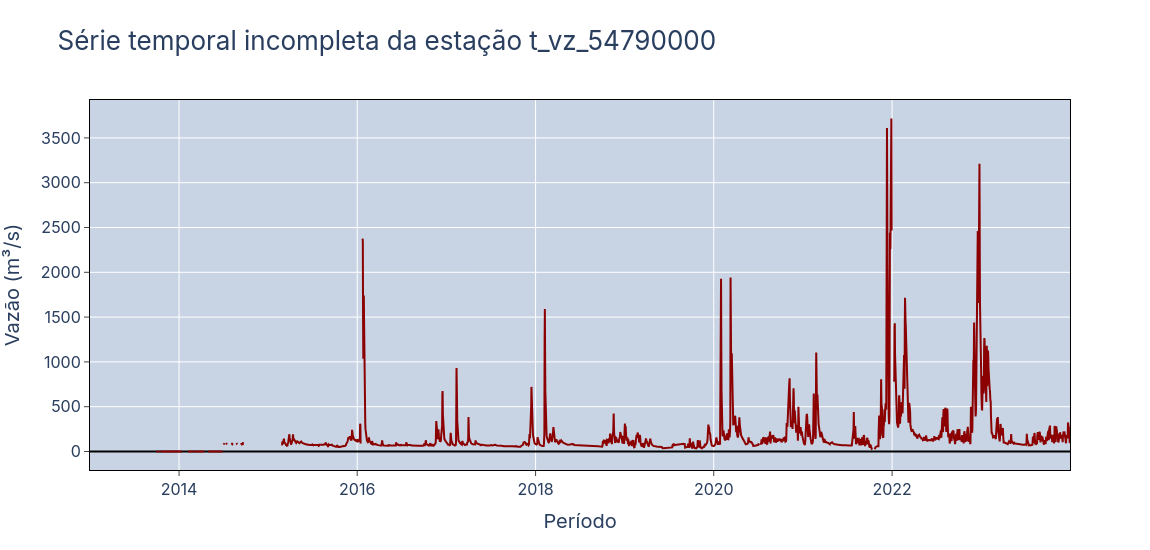
\includegraphics[scale=0.25]{Figuras/jequiti/jequitinhonhaSerieIncompleta_t_vz_54790000.png}
	\caption{Série temporal incompleta da estação t\_vz\_54790000 (fonte: o autor)}
	\label{fig:jequitinhonhaSerieIncompleta_t_vz_54790000}
\end{figure}

A seguir, destaca-se o trecho da série com a maior quantidade de dados faltantes (figura \ref{fig:jequitinhonhaSerieIncompleta_t_vz_54790000-2013_2016}), que abrange o período de janeiro de 2013 a janeiro de 2016. Em sequência, é apresentada a série após a imputação dos dados (figura \ref{fig:jequitinhonhaSerieCompleta_t_vz_54790000-2013_2016}). Notavelmente, essa seção não apresentou resultados ideais, uma vez que a imputação atribuiu vazões zero em vários dias, o que não é realista, pois isso indicaria a secagem completa do rio, o que é improvável. No entanto, esses valores zero não impactaram significativamente os resultados finais da análise, já que se referem a um período distante do foco principal deste estudo. Uma alternativa seria excluir todo o trecho anterior ao ano de 2016, mas optou-se por manter a uniformidade nos critérios de aproveitamento dos dados ao longo do trabalho, dado que outros rios também foram analisados, e buscava-se assegurar consistência nos resultados.

\begin{figure}[!h]
	\centering
	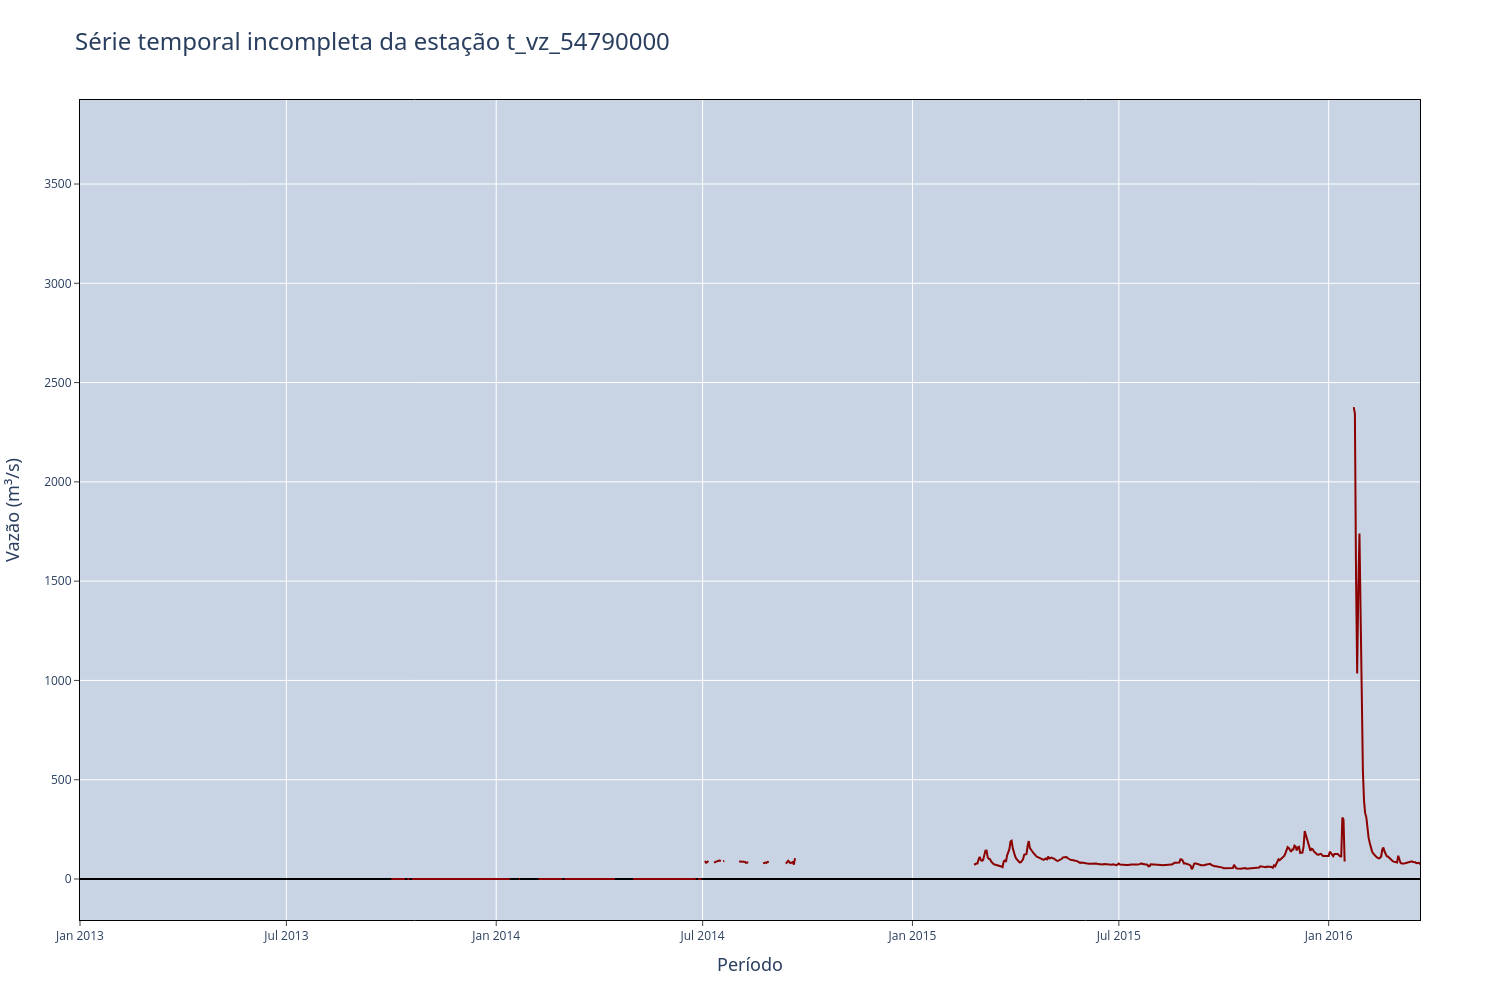
\includegraphics[scale=0.25]{Figuras/jequiti/jequitinhonhaSerieIncompleta_t_vz_54790000-2013_2016.png}
	\caption{Detalhe da série temporal da estação t\_vz\_54790000, ainda sem dados imputados, de 2013 a 2016 (fonte: o autor)}
	\label{fig:jequitinhonhaSerieIncompleta_t_vz_54790000-2013_2016}
\end{figure}

\begin{figure}[!h]
	\centering
	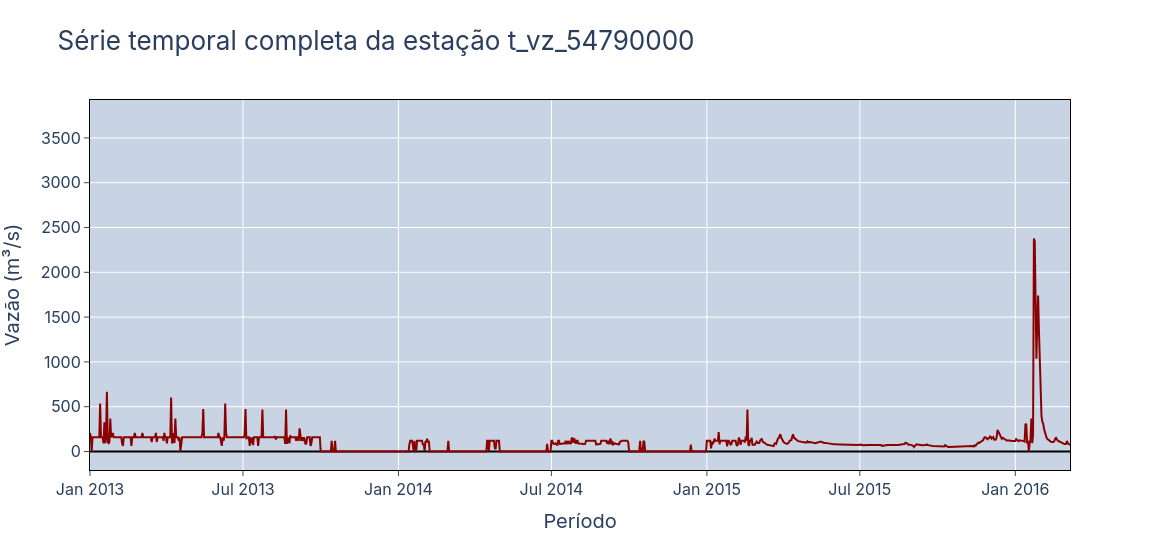
\includegraphics[scale=0.25]{Figuras/jequiti/jequitinhonhaSerieCompleta_t_vz_54790000-2013_2016.png}
	\caption{Detalhe da série temporal da estação t\_vz\_54790000, com dados imputados, de 2013 a 2016 (fonte: o autor)}
	\label{fig:jequitinhonhaSerieCompleta_t_vz_54790000-2013_2016}
\end{figure}

Observe também o trecho de dados faltantes mais próximo ao final dos anos analisados, em 2021 e 2022 (figura \ref{fig:jequitinhonhaSerieIncompleta_t_vz_54790000-2021_2022}). Esta porção da série ficou boa visto que havia informação prévia suficiente, a inserção de dados respeitou coerentemente a sazonalidade (figura \ref{fig:jequitinhonhaSerieCompleta_t_vz_54790000-2021_2022}).

\begin{figure}[!h]
	\centering
	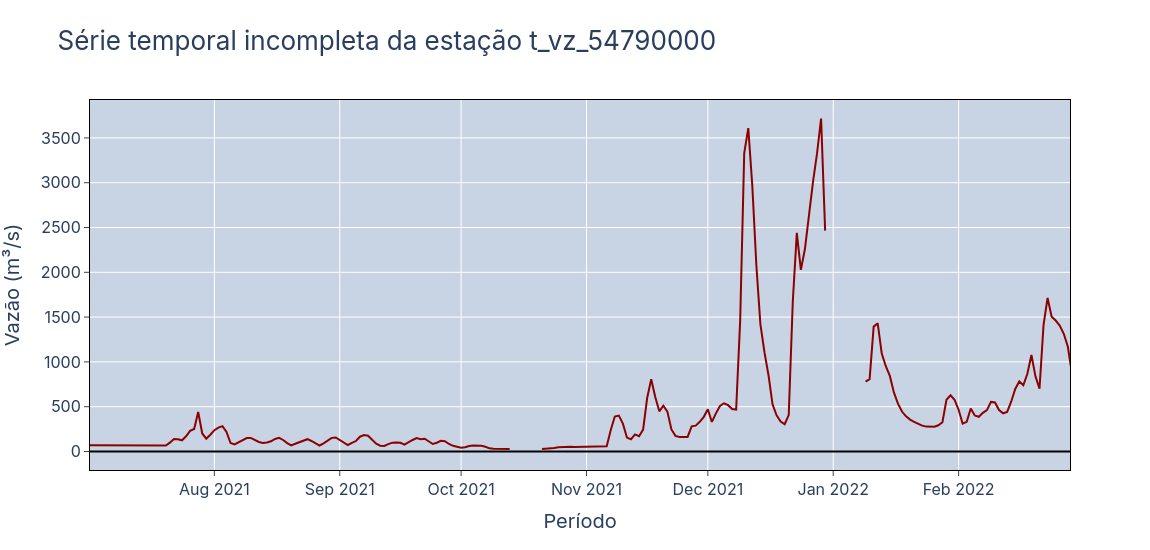
\includegraphics[scale=0.25]{Figuras/jequiti/jequitinhonhaSerieIncompleta_t_vz_54790000-2021_2022.png}
	\caption{Série temporal incompleta da estação t\_vz\_54790000 no detalhe entre 2021 e 2022 (fonte: o autor)}
	\label{fig:jequitinhonhaSerieIncompleta_t_vz_54790000-2021_2022}
\end{figure}

\begin{figure}[!h]
	\centering
	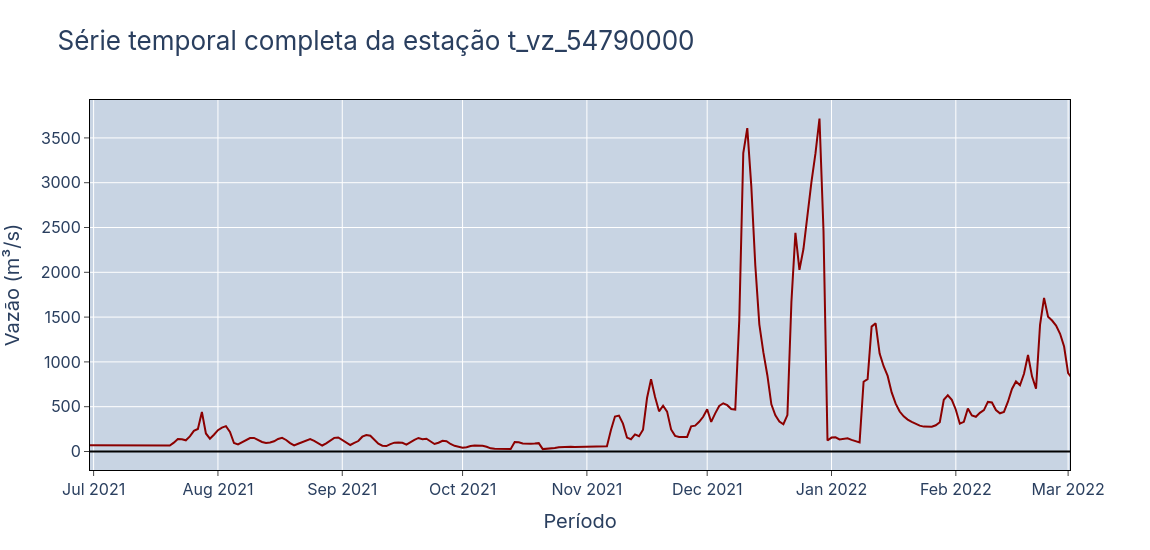
\includegraphics[scale=0.25]{Figuras/jequiti/jequitinhonhaSerieCompleta_t_vz_54790000-2021_2022.png}
	\caption{Série temporal completa da estação t\_vz\_54790000 no detalhe entre 2021 e 2022 (fonte: o autor)}
	\label{fig:jequitinhonhaSerieCompleta_t_vz_54790000-2021_2022}
\end{figure}

Por fim, uma visão ampla de como ficou a série temporal após os procedimentos de imputar os dados. (figura \ref{fig:jequitinhonhaSerieCompleta_t_vz_54790000})

\begin{figure}[!h]
	\centering
	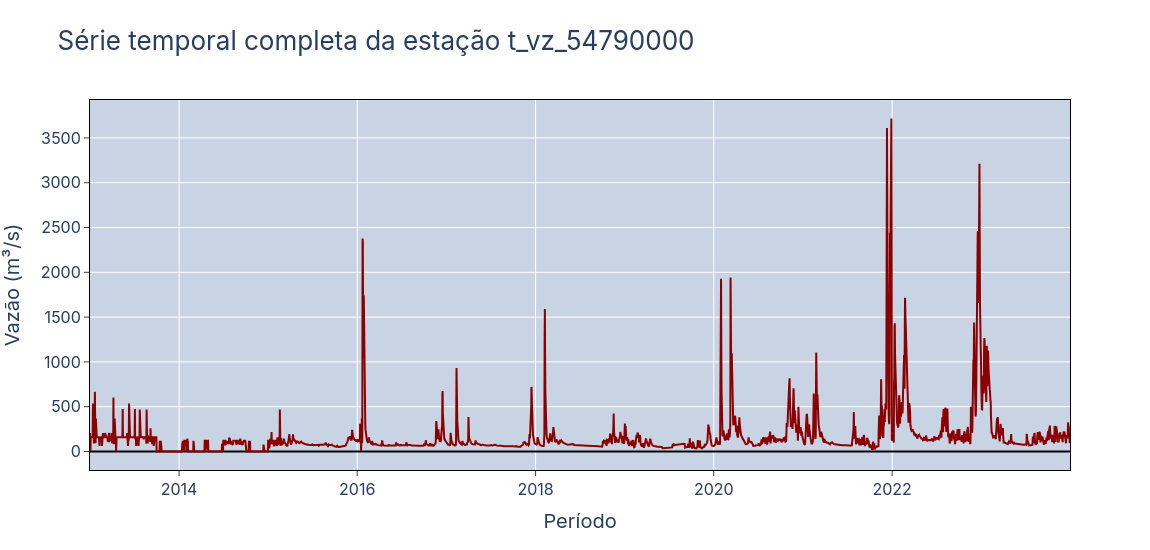
\includegraphics[scale=0.25]{Figuras/jequiti/jequitinhonhaSerieCompleta_t_vz_54790000.png}
	\caption{Série temporal completa da estação t\_vz\_54790000 (fonte: o autor)}
	\label{fig:jequitinhonhaSerieCompleta_t_vz_54790000}
\end{figure}

A mesma análise foi realizada para as estações de chuva. Na estação t\_cv\_54790000 (figura \ref{fig:jequitinhonhaSerieIncompleta_t_cv_54790000}) faltavam 273 dias de dados (6,79\%). Já a estação t\_cv\_01640000 estava totalmente preenchida, sem valores nulos. (figura \ref{fig:jequitinhonhaSerieCompleta_t_cv_01640000})

\begin{figure}[!h]
	\centering
	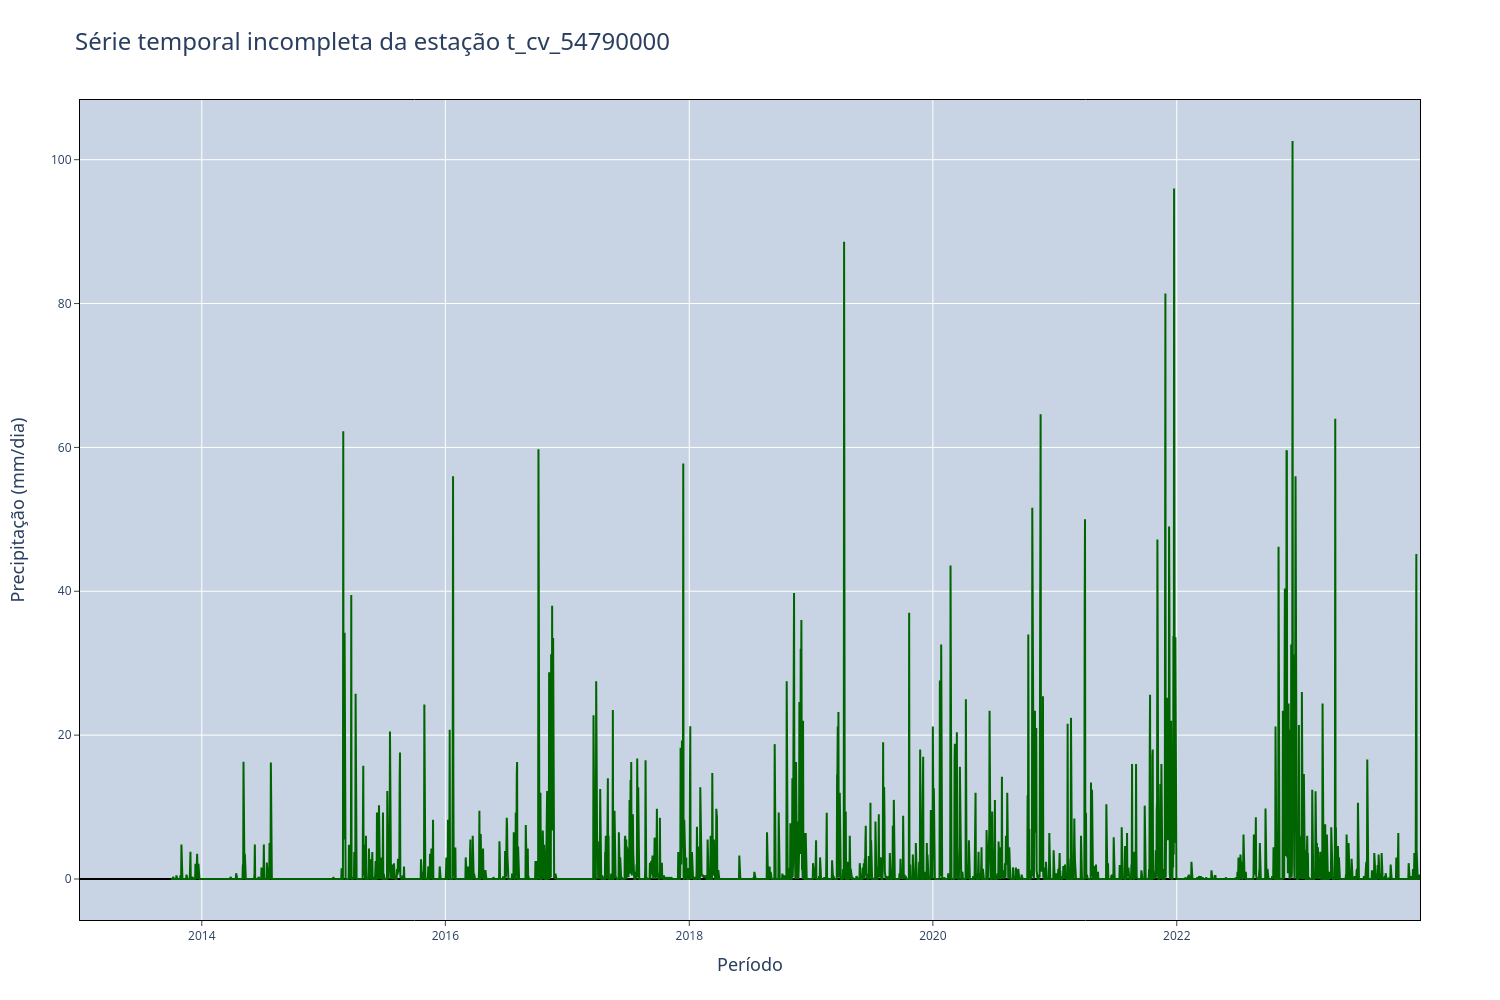
\includegraphics[scale=0.25]{Figuras/jequiti/jequitinhonhaSerieIncompleta_t_cv_54790000.png}
	\caption{Série temporal incompleta da estação t\_cv\_54790000 (fonte: o autor)}
	\label{fig:jequitinhonhaSerieIncompleta_t_cv_54790000}
\end{figure}

Note que no início desta série de precipitação, o ano de 2013, não possuem dados. As séries de chuva completas ficaram desta forma (figuras \ref{fig:jequitinhonhaSerieCompleta_t_cv_54790000} e \ref{fig:jequitinhonhaSerieCompleta_t_cv_01640000})

\begin{figure}[!h]
	\centering
	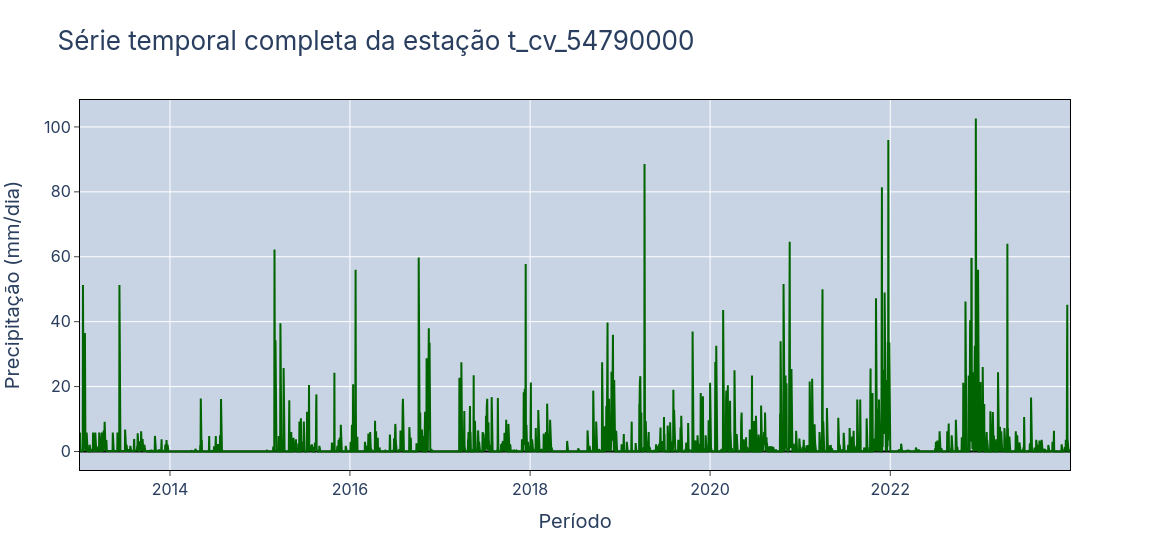
\includegraphics[scale=0.25]{Figuras/jequiti/jequitinhonhaSerieCompleta_t_cv_54790000.png}
	\caption{Série temporal completa da estação t\_cv\_54790000 (fonte: o autor)}
	\label{fig:jequitinhonhaSerieCompleta_t_cv_54790000}
\end{figure}

\begin{figure}[!h]
	\centering
	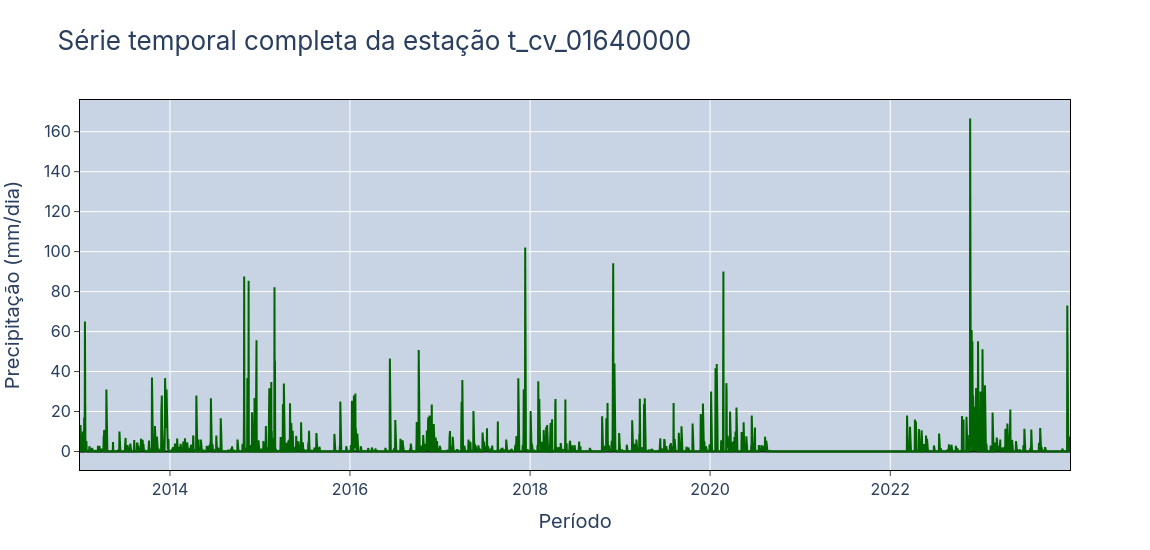
\includegraphics[scale=0.25]{Figuras/jequiti/jequitinhonhaSerieCompleta_t_cv_01640000.png}
	\caption{Série temporal completa da estação t\_cv\_01640000 (fonte: o autor)}
	\label{fig:jequitinhonhaSerieCompleta_t_cv_01640000}
\end{figure}

\subsection{Rio Doce}

A estação alvo para o rio Doce é a estação c\_vz\_56994500. Sua série temporal foi a que apresentou melhor qualidade no que diz respeito à frequência de medições realizadas. Havia falta de apenas 3 dias, dos 4017 dias do período inteiro. Apenas o preenchimento sazonal bastou para completar a série e não foi preciso mais que isso. Cabe destacar a sazonalidade da série. Ficou bastante evidente este comportamento. (figura \ref{fig:doceSerieCompleta_c_vz_56994500})

\begin{figure}[!h]
	\centering
	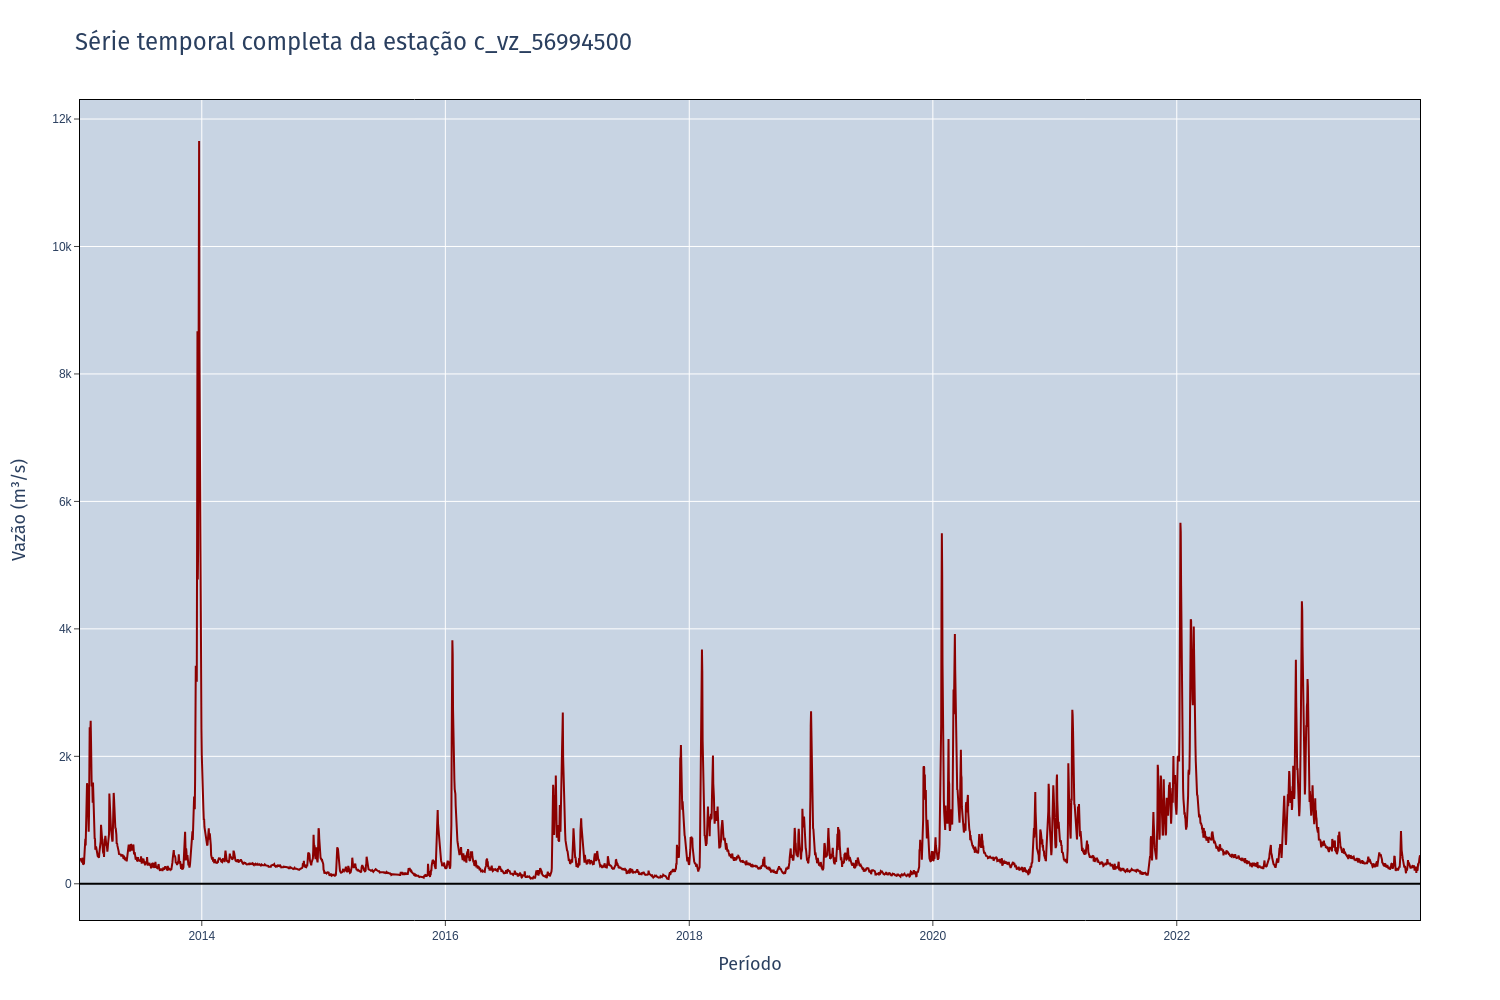
\includegraphics[scale=0.25]{Figuras/rio_doce/doceSerieCompleta_c_vz_56994500.png}
	\caption{Série temporal completa da estação c\_vz\_56994500 (fonte: o autor)}
	\label{fig:doceSerieCompleta_c_vz_56994500}
\end{figure}

Se para os dados de vazão no rio Doce a série foi, digamos, mais comportada, o mesmo não se pode dizer exatamente das estações de chuva. Ao menos, não para duas delas. Estas estações tiveram os dados desconsiderados e foram removidos das análises. Primeiro foi a estação t\_cv\_56990850 que possuía valores discrepantes demais para serem considerados. Valores da ordem de 7000 mm/dia, 8500 mm/dia. Além deste problema, havia ainda 3134 dias com dados nulos, o que representava 78\% do total. (figura \ref{fig:doceSerieIncompleta_t_cv_56990850})

A outra estação removida foi a t\_cv\_56994500. Conforme pode ser observado na figura \ref{fig:doceSerieCompleta_t_cv_56994500}, nela havia um longo hiato de dados zerados, voltando à normalidade apenas mais recentemente. Como as informações de precipitação que deveria haver para a estação no período do hiato, pode ser retirado de outras estações usadas na modelagem, optou-se por remover esta estação completamente do trabalho.

\begin{figure}[!h]
	\centering
	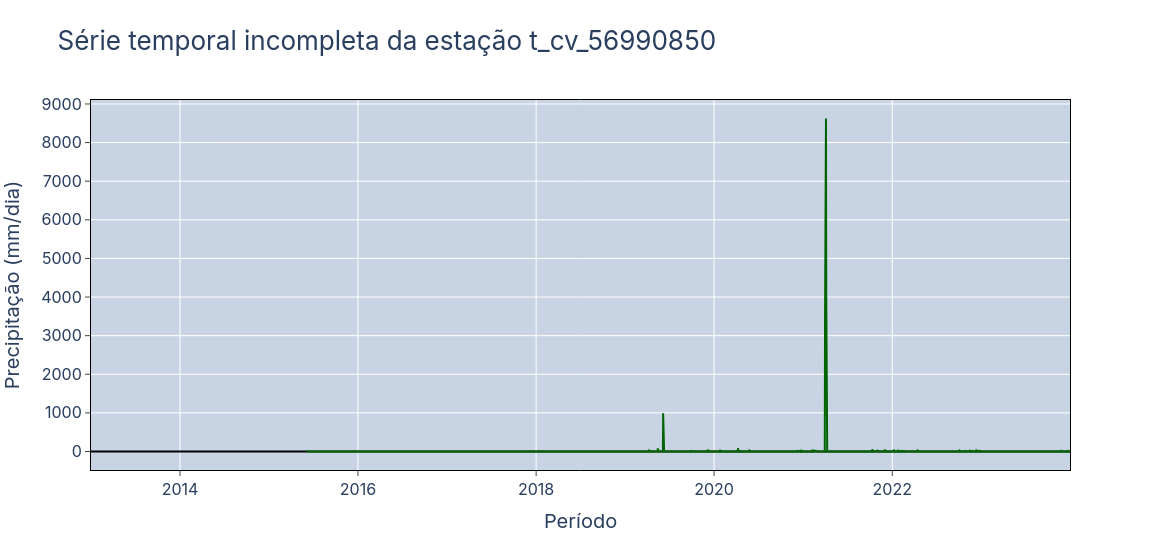
\includegraphics[scale=0.25]{Figuras/rio_doce/doceSerieIncompleta_t_cv_56990850.png}
	\caption{Série temporal da estação t\_cv\_56990850 - não utilizada (fonte: o autor)}
	\label{fig:doceSerieIncompleta_t_cv_56990850}
\end{figure}

\begin{figure}[!h]
	\centering
	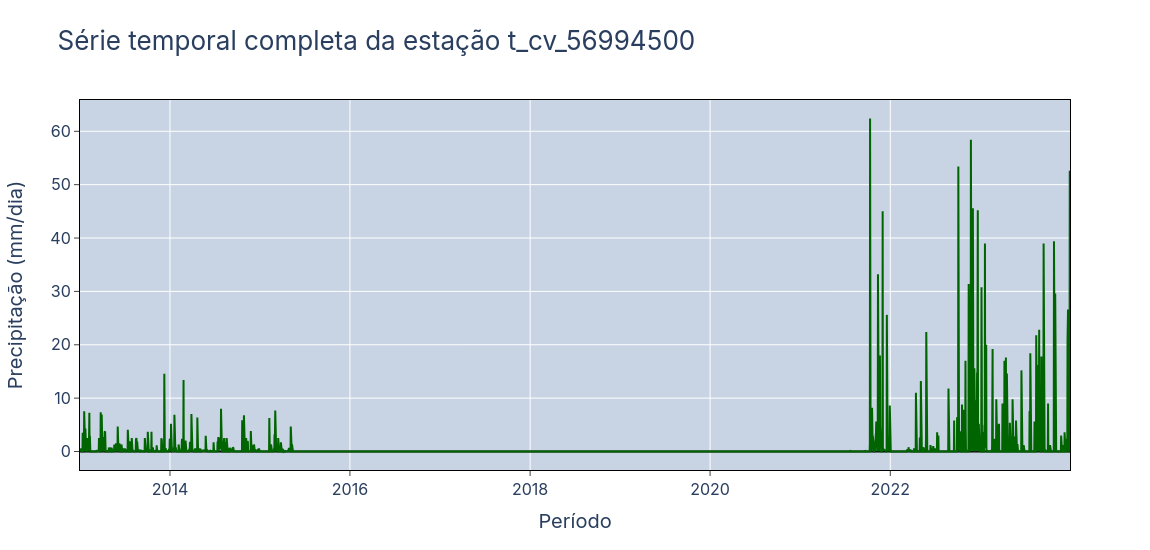
\includegraphics[scale=0.25]{Figuras/rio_doce/doceSerieCompleta_t_cv_56994500.png}
	\caption{Série temporal da estação t\_cv\_56994500 - não utilizada (fonte: o autor)}
	\label{fig:doceSerieCompleta_t_cv_56994500}
\end{figure}

As estações que, enfim, foram empregadas na modelagem são as que estão na tabela e, adiante, o gráfico da série temporal de cada uma delas. (figuras \ref{fig:doceSerieCompleta_c_cv_01941010}, \ref{fig:doceSerieCompleta_c_cv_01941004}, \ref{fig:doceSerieCompleta_c_cv_01941006} e \ref{fig:doceSerieCompleta_t_cv_56990005})

\begin{table}[h!]
	\centering \small
	\caption{Estações de precipitação usadas - final}
	\begin{tabular}{|c|c|c|} \hline
		\textbf{Estação} & \textbf{\# dados faltantes} & \textbf{\% dados faltantes} \\ \hline
		c\_cv\_01941010  & 153                         & 3,81 \\ \hline
		c\_cv\_01941004  & 31                          & 0,77 \\ \hline
		c\_cv\_01941006  & 0                           & 0,00 \\ \hline
		t\_cv\_56990005  & 1395                        & 34,73 \\ \hline
	\end{tabular}
	\label{tab:estacoes_chuva_usadas_final_rio_doce}
\end{table}

\begin{figure}[!h]
	\centering
	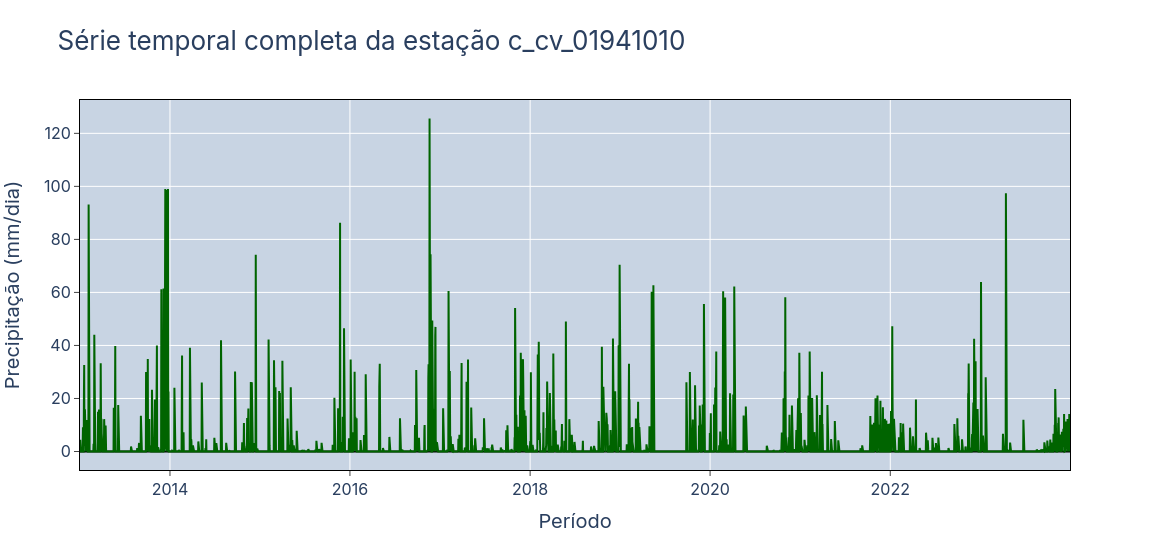
\includegraphics[scale=0.25]{Figuras/rio_doce/doceSerieCompleta_c_cv_01941010.png}
	\caption{Série temporal completa da estação c\_cv\_01941010 (fonte: o autor)}
	\label{fig:doceSerieCompleta_c_cv_01941010}
\end{figure}

\begin{figure}[!h]
	\centering
	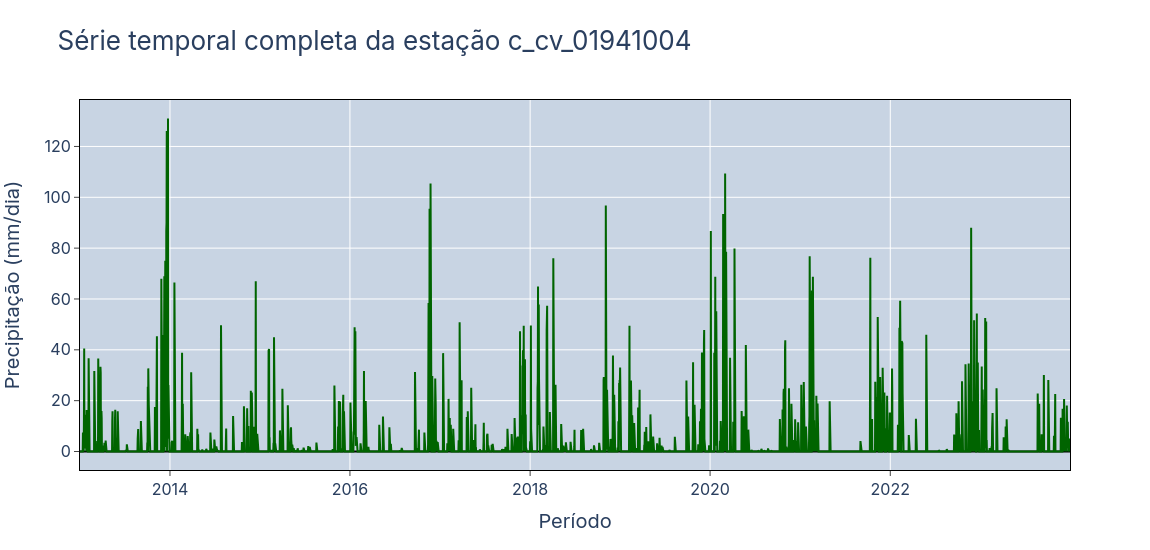
\includegraphics[scale=0.25]{Figuras/rio_doce/doceSerieCompleta_c_cv_01941004.png}
	\caption{Série temporal completa da estação c\_cv\_01941004 (fonte: o autor)}
	\label{fig:doceSerieCompleta_c_cv_01941004}
\end{figure}

\begin{figure}[!h]
	\centering
	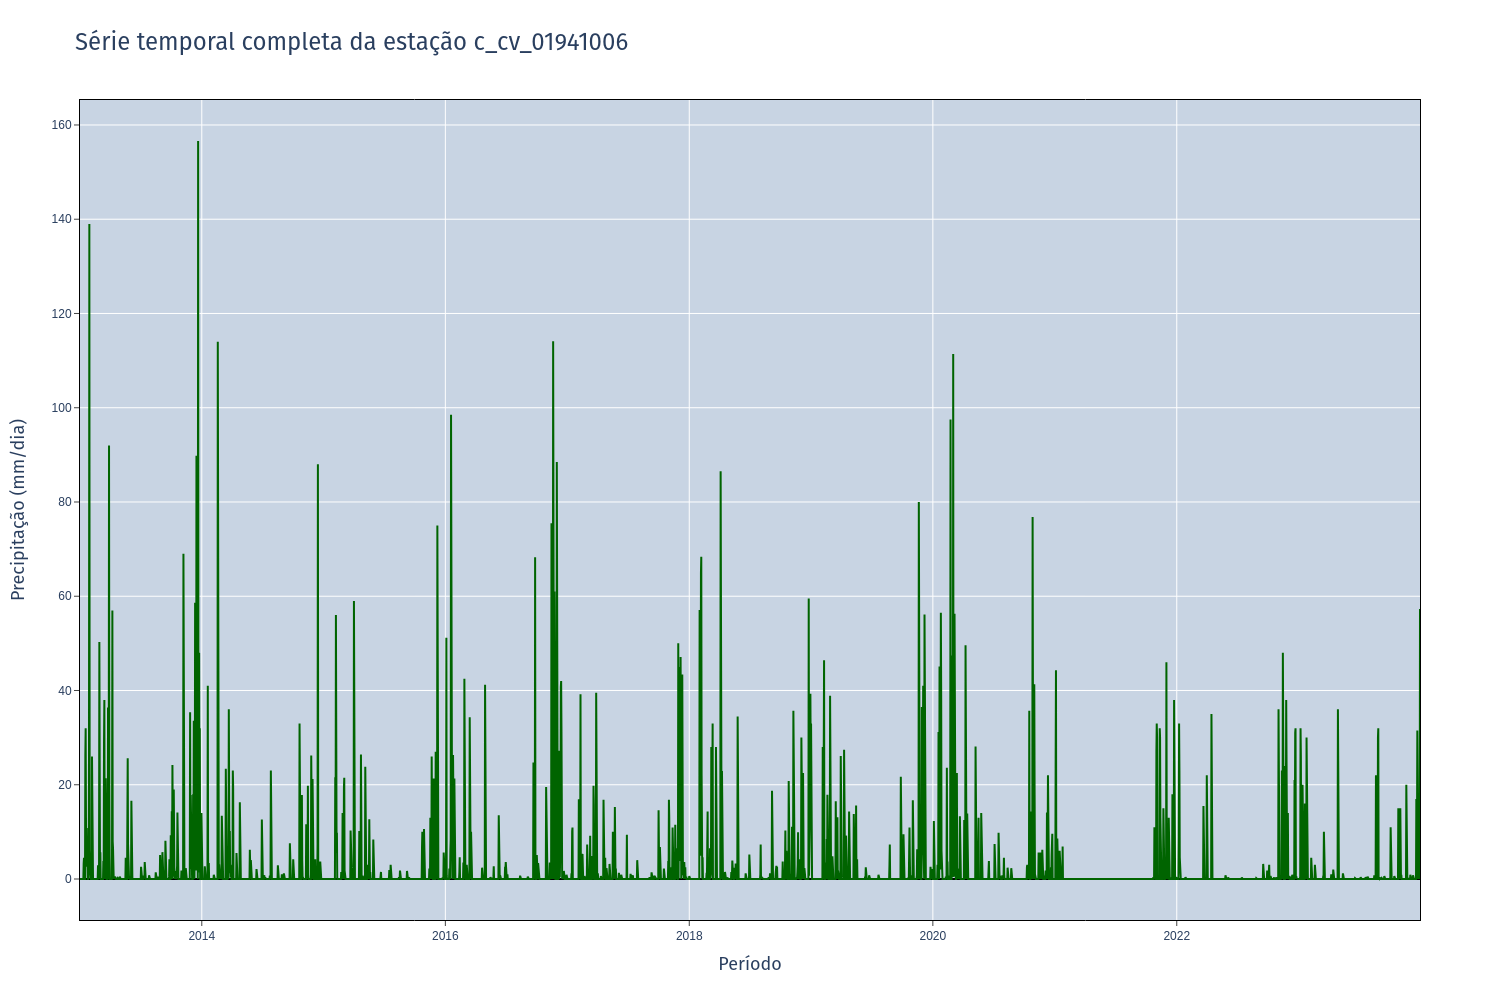
\includegraphics[scale=0.25]{Figuras/rio_doce/doceSerieCompleta_c_cv_01941006.png}
	\caption{Série temporal completa da estação c\_cv\_01941006 (fonte: o autor)}
	\label{fig:doceSerieCompleta_c_cv_01941006}
\end{figure}

\begin{figure}[!h]
	\centering
	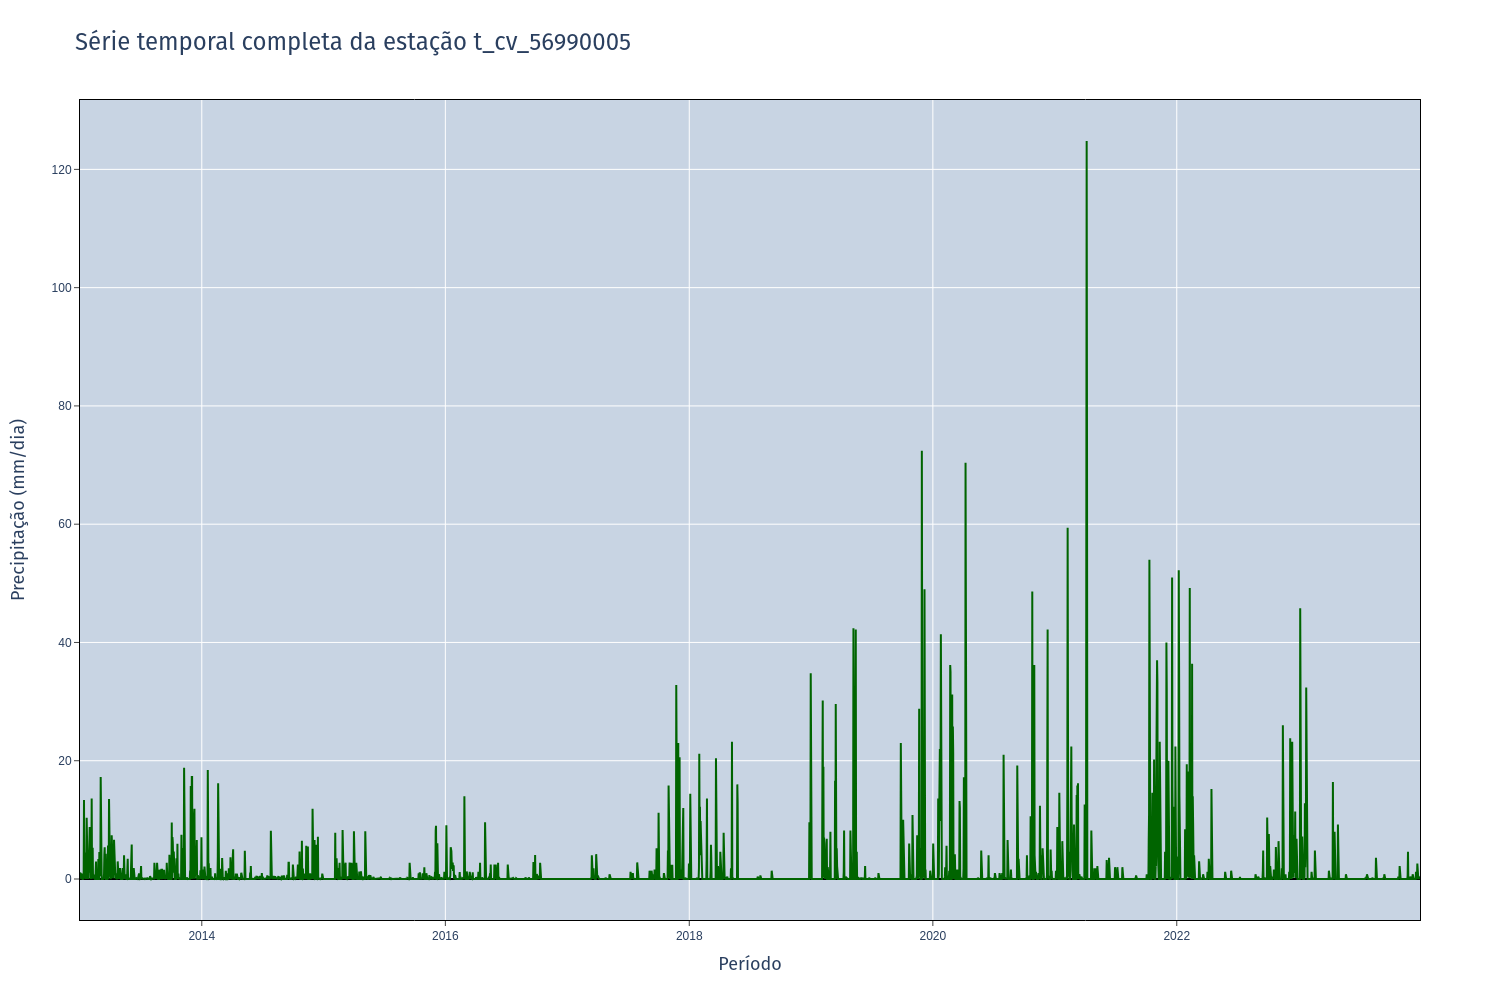
\includegraphics[scale=0.25]{Figuras/rio_doce/doceSerieCompleta_t_cv_56990005.png}
	\caption{Série temporal completa da estação t\_cv\_56990005 (fonte: o autor)}
	\label{fig:doceSerieCompleta_t_cv_56990005}
\end{figure}

\subsection{Rio Grande}

O rio Grande apresentou desafios significativos ao longo de todo o desenvolvimento deste trabalho. A dificuldade inicial surgiu na ausência de dados disponíveis em estações dentro do estado de Minas Gerais para o período de análise estipulado, conforme mencionado anteriormente. Foi necessário buscar uma estação o mais próxima possível da divisa com Minas Gerais, localizada no estado de São Paulo, especificamente no município de Ilha Solteira. Entretanto, os desafios não se limitaram a essa questão geográfica.

A série temporal de vazão da estação selecionada, denominada t\_vz\_62020080, estava incompleta e não abrangia todo o período de 11 anos estipulado para a análise. (figura \ref{fig:grandeSerieIncompleta_t_vz_62020080}) Os dados disponíveis mais antigos datavam de 2020. Contudo, em conformidade com o escopo estabelecido para este estudo, foi realizado o preenchimento dos dados faltantes, aplicando-se o mesmo protocolo utilizado para os demais rios analisados. Este procedimento foi necessário para garantir a consistência, integridade e comparabilidade das análises subsequentes.

\begin{figure}[!h]
	\centering
	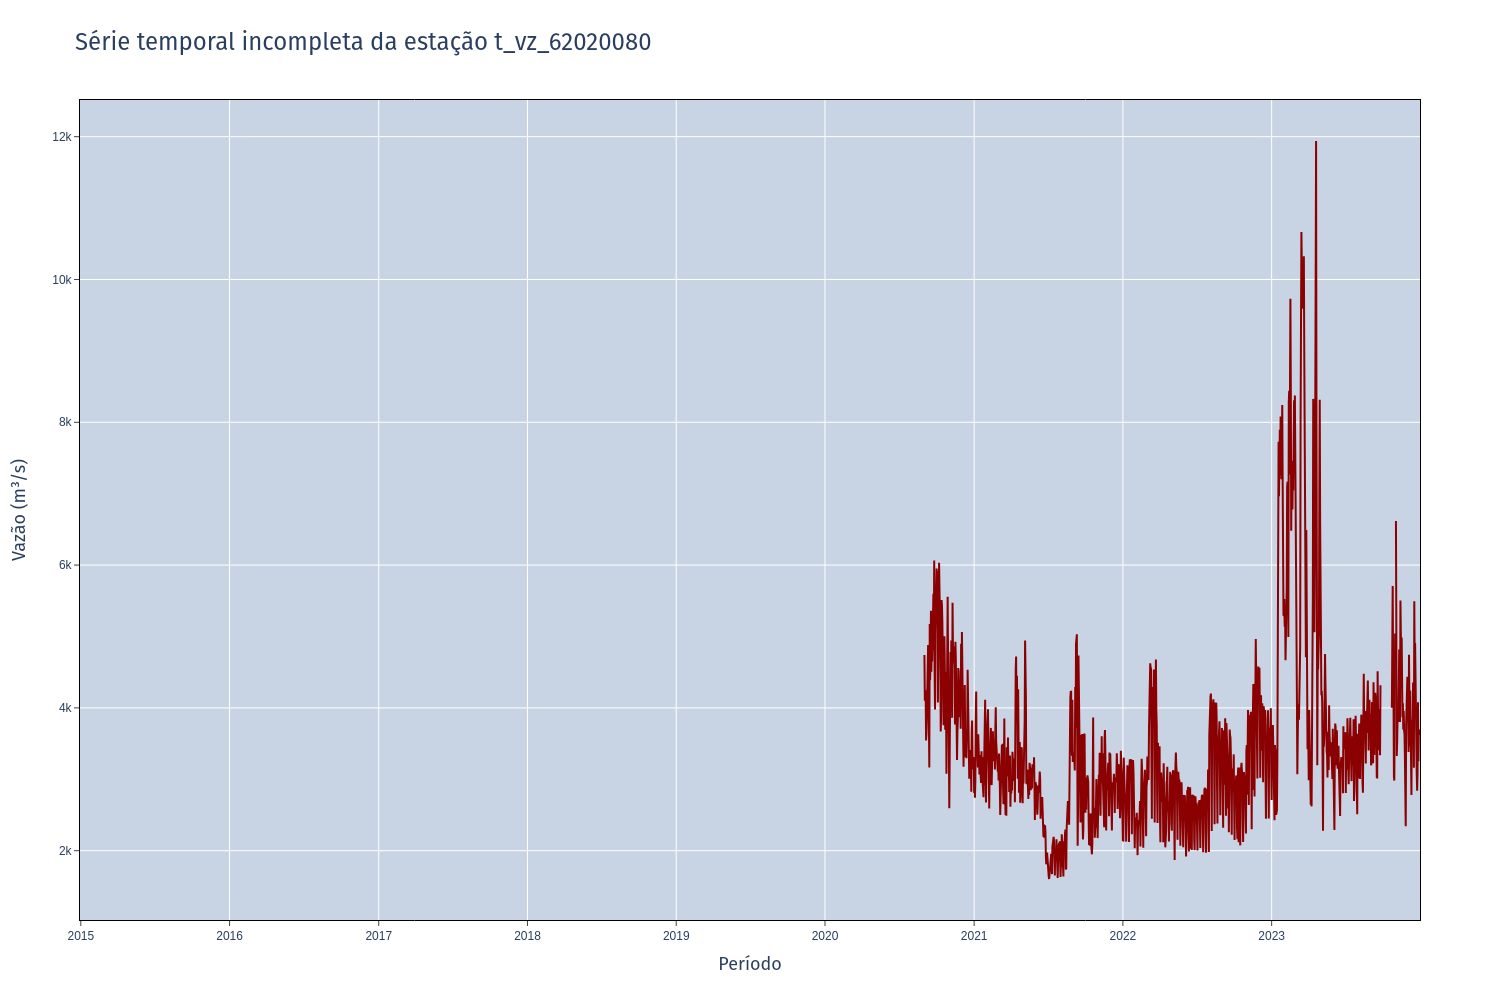
\includegraphics[scale=0.25]{Figuras/rio_grande/grandeSerieIncompleta_t_vz_62020080.png}
	\caption{Série temporal incompleta da estação t\_vz\_62020080 (fonte: o autor)}
	\label{fig:grandeSerieIncompleta_t_vz_62020080}
\end{figure}

Infelizmente, o caráter ruidoso da série permaneceu mesmo após a aplicação do protocolo de preenchimento dos dados ausentes, conforme pode ser observado na imagem final gerada. (figura \ref{fig:grandeSerieCompleta_t_vz_62020080}) A série em questão apresentava 2099 dias faltantes, correspondendo a aproximadamente 64\% de dados nulos. Outro aspecto relevante para essa estação é que, diferentemente das outras, não foram utilizados os 4.017 registros previstos inicialmente. As informações mais antigas disponíveis datavam de 2015, resultando, assim, em um total de 3289 registros diários utilizados especificamente para o rio Grande.

\begin{figure}[!h]
	\centering
	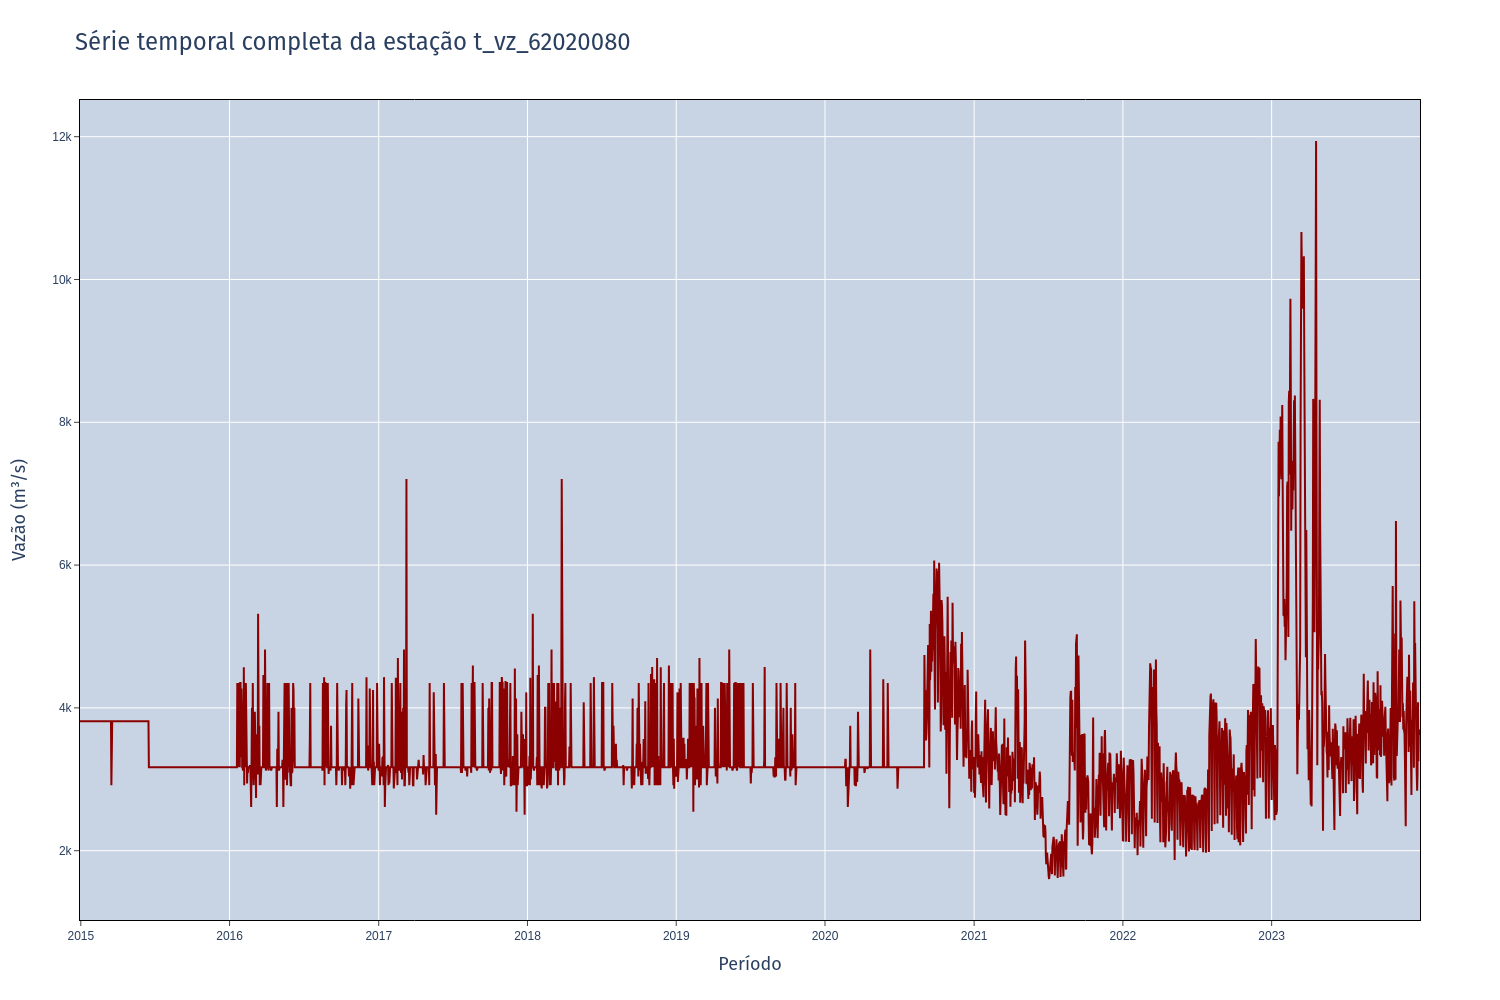
\includegraphics[scale=0.25]{Figuras/rio_grande/grandeSerieCompleta_t_vz_62020080.png}
	\caption{Série temporal completa da estação t\_vz\_62020080 (fonte: o autor)}
	\label{fig:grandeSerieCompleta_t_vz_62020080}
\end{figure}

A estação de precipitação utilizada, a única neste caso, foi a estação t\_cv\_61998080, pois foi a única que apresentou dados válidos. Curiosamente, outra estação de precipitação disponível também apresentou dados para o período analisado, mas a base de dados consistia exclusivamente em valores zero. Por essa razão, a estação t\_cv\_62020080 foi completamente excluída do estudo.

Em relação à estação t\_cv\_61998080, houve necessidade de preencher apenas um número reduzido de dados ausentes, totalizando 169 registros, o que correspondia a 5,14\% do total. (figura \ref{fig:grandeSerieCompleta_t_cv_61998080}) Trata-se de uma série com uma quantidade expressiva de dados, que efetivamente pôde contribuir de maneira significativa para as análises realizadas.

\begin{figure}[!h]
	\centering
	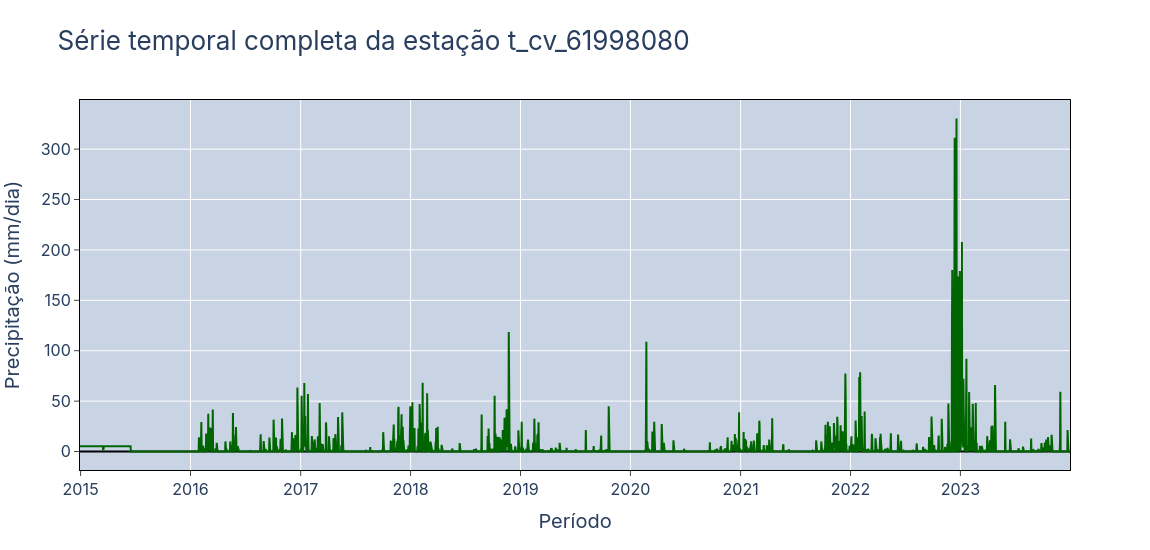
\includegraphics[scale=0.25]{Figuras/rio_grande/grandeSerieCompleta_t_cv_61998080.png}
	\caption{Série completa da estação t\_cv\_61998080 (fonte: o autor)}
	\label{fig:grandeSerieCompleta_t_cv_61998080}
\end{figure}

Ressalta-se que o trecho de dados faltantes para a estação t\_cv\_61998080 concentrava-se no início da série temporal, especificamente no ano de 2015. No gráfico os dados já estão imputados.

\subsection{Rio São Francisco}

Por fim, foi realizado o procedimento de preenchimento dos dados nulos para o Rio São Francisco. A estação-alvo c\_vz\_44290002 apresentou uma série bastante completa ao longo do período de análise, com apenas 120 dias nulos em um total de 4017 dias. O trecho com dados faltantes pode ser observado em detalhe na figura (\ref{fig:franciscoSerieIncompleta_c_vz_44290002-detalhe}).

Para esta estação, o preenchimento sazonal foi suficiente para suprir as lacunas existentes, não sendo necessário aplicar procedimentos adicionais de imputação de dados. (figura \ref{fig:franciscoSerieCompleta_c_vz_44290002})

\begin{figure}[!h]
	\centering
	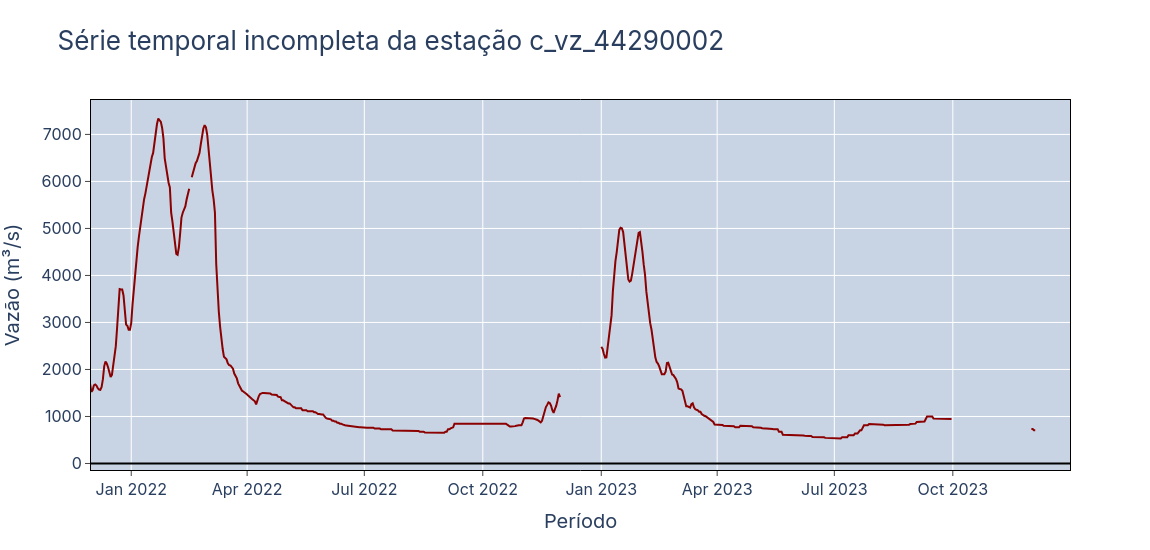
\includegraphics[scale=0.25]{Figuras/rio_sao_francisco/franciscoSerieIncompleta_c_vz_44290002-detalhe.png}
	\caption{Detalhe do trecho com dados nulos da estação c\_vz\_44290002 (fonte: o autor)}
	\label{fig:franciscoSerieIncompleta_c_vz_44290002-detalhe}
\end{figure}

\begin{figure}[!h]
	\centering
	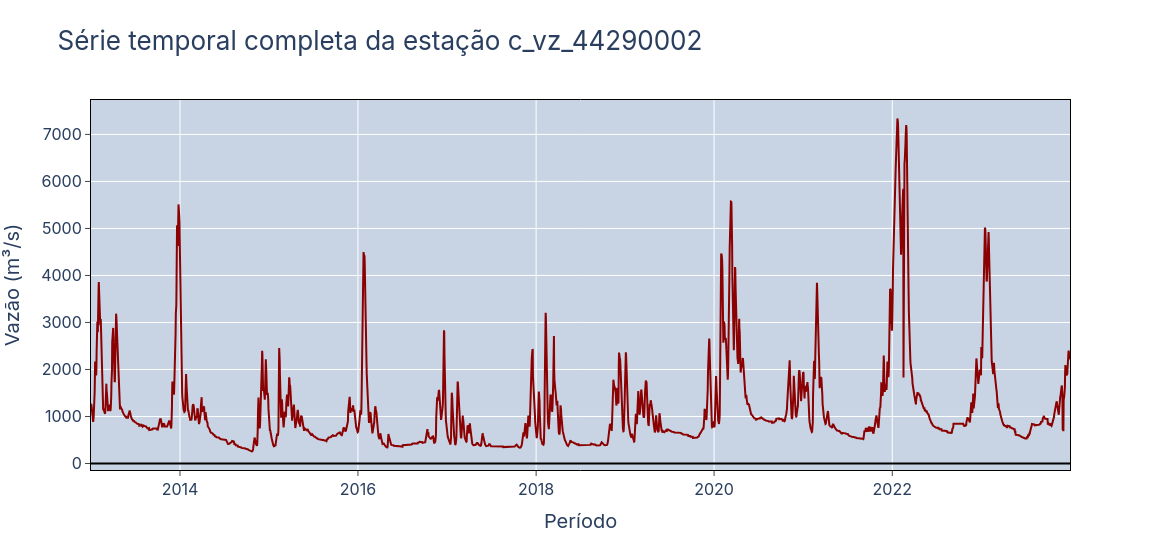
\includegraphics[scale=0.25]{Figuras/rio_sao_francisco/franciscoSerieCompleta_c_vz_44290002.png}
	\caption{Série temporal completa da estação c\_vz\_44290002 (fonte: o autor)}
	\label{fig:franciscoSerieCompleta_c_vz_44290002}
\end{figure}

No que se refere às estações de precipitação selecionadas para a análise no rio São Francisco, não foi necessário realizar nenhuma inserção de dados, uma vez que todas as séries estavam completas, abrangendo a totalidade dos 4017 dias de registro. As séries temporais correspondentes podem ser visualizadas nos gráficos apresentados a seguir. (figuras \ref{fig:franciscoSerieCompleta_c_cv_01544017}, \ref{fig:franciscoSerieCompleta_c_cv_01544032}, \ref{fig:franciscoSerieCompleta_c_cv_01544036})

\begin{figure}[!h]
	\centering
	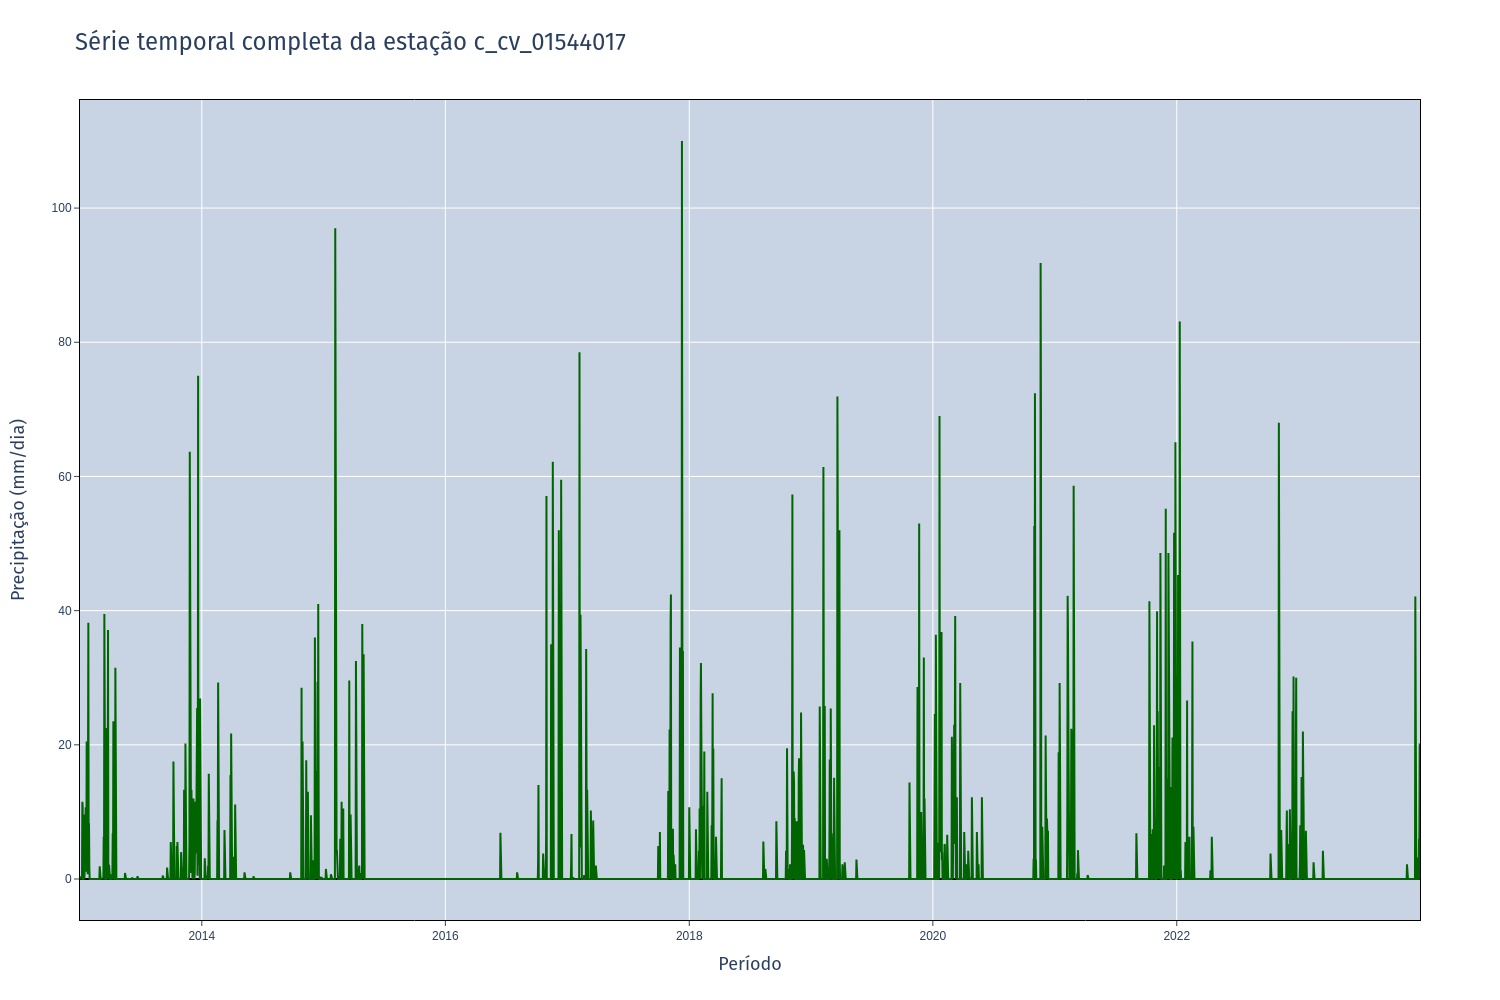
\includegraphics[scale=0.25]{Figuras/rio_sao_francisco/franciscoSerieCompleta_c_cv_01544017.png}
	\caption{Série temporal completa da estação c\_cv\_01544017 (fonte: o autor)}
	\label{fig:franciscoSerieCompleta_c_cv_01544017}
\end{figure}

\begin{figure}[!h]
	\centering
	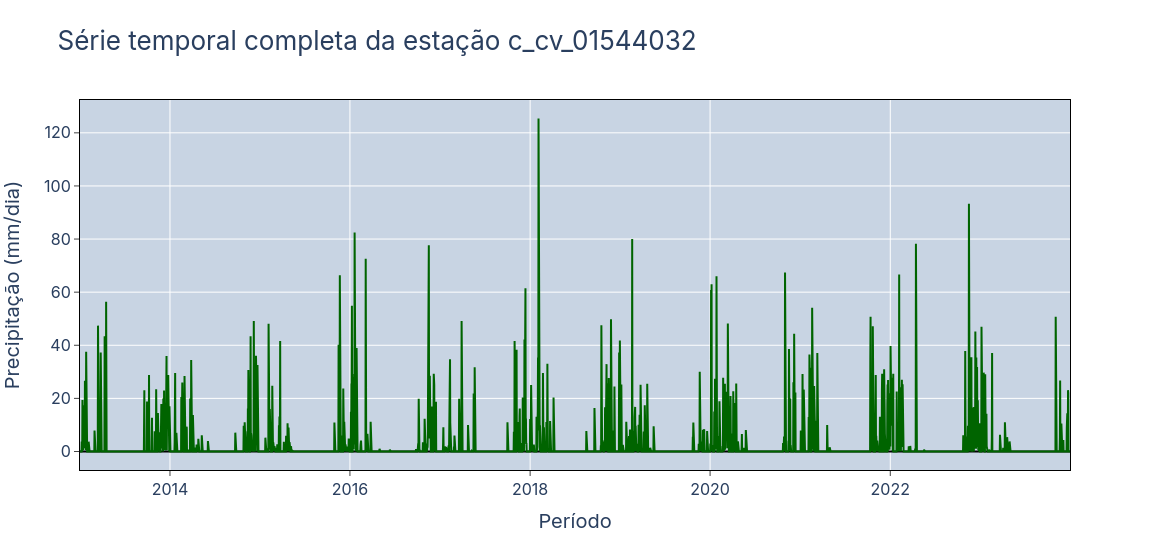
\includegraphics[scale=0.25]{Figuras/rio_sao_francisco/franciscoSerieCompleta_c_cv_01544032.png}
	\caption{Série temporal completa da estação c\_cv\_01544032 (fonte: o autor)}
	\label{fig:franciscoSerieCompleta_c_cv_01544032}
\end{figure}

\begin{figure}[!h]
	\centering
	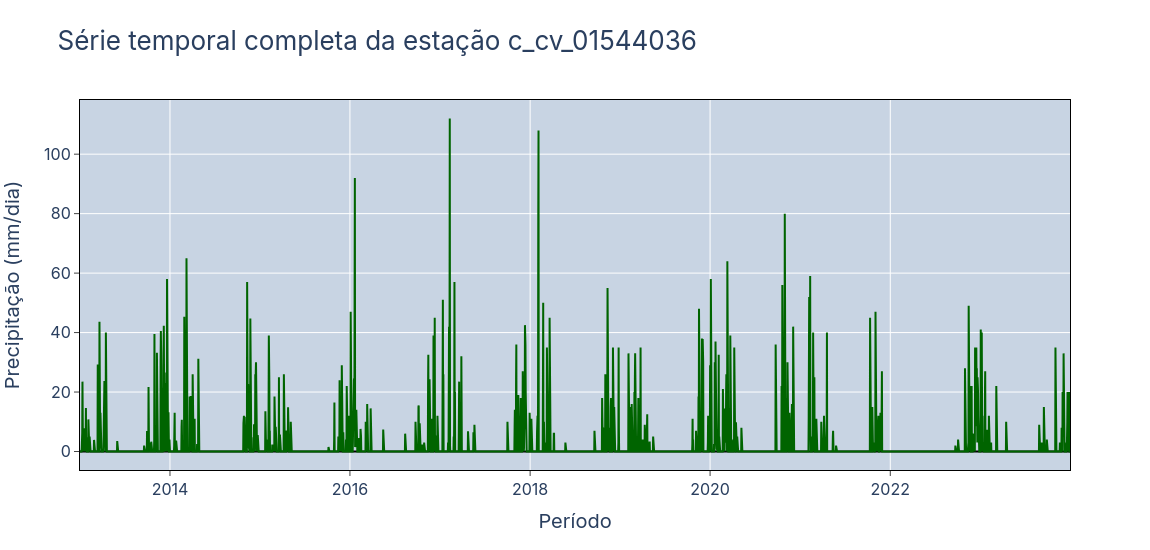
\includegraphics[scale=0.25]{Figuras/rio_sao_francisco/franciscoSerieCompleta_c_cv_01544036.png}
	\caption{Série temporal completa da estação c\_cv\_01544036 (fonte: o autor)}
	\label{fig:franciscoSerieCompleta_c_cv_01544036}
\end{figure}

\section{Variáveis Utilizadas}
%Listar e explicar as variáveis contínuas e categóricas utilizadas nos modelos.

As variáveis do trabalho, exceto as categóricas, obviamente, são todas contínuas. Todas as séries temporais foram ajustadas para estarem completas dentro do período trabalhado, totalizando 4017 registros diários. A exceção ficou por conta dos dados do rio Grande, em que o dado mais antigo foi o dia 30 de dezembro de 2014.

Para que se tenha uma noção melhor, abaixo seguem alguns dados estatísticos relevantes que informam sobre os dados de vazão e precipitação utilizados. Conste-se que as unidades de precipitação estão em mm/dia e vazão em $m^3/s$.

\begin{table}[!h]
	\centering \small
	\caption{Rio Jequitinhonha}
	\begin{tabular}{|l|r|r|r|r|r|r|} \hline 
		\textbf{Variável}   & \textbf{\#} & \textbf{Média} & \textbf{Desvio-padrão} & \textbf{Mín} & \textbf{< 50\%} & \textbf{Máx} \\\hline
		t\_cv\_01640000     & 4017        & 1,58           & 6,85                   & 0,00         & 0,00            & 166,60       \\\hline
		t\_cv\_54790000     & 4017        & 1,68           & 6,31                   & 0,00         & 0,00            & 102,60       \\\hline
		t\_vz\_54790000 (y) & 4017        & 160,95         & 267,90                 & 0,00         & 95,95           & 3716,65      \\\hline
	\end{tabular}
	\label{tab:variaveis_jequitinhonha}
\end{table}

\begin{table}[!h]
	\centering \small
	\caption{Rio Doce}
	\begin{tabular}{|l|r|r|r|r|r|r|} \hline 
		\textbf{Variável}   & \textbf{\#} & \textbf{Média} & \textbf{Desvio-padrão} & \textbf{Mín} & \textbf{< 50\%} & \textbf{Máx} \\\hline
		c\_cv\_01941010     & 4017        & 2,21           & 8,41                   & 0,00         & 0,00            & 125,60       \\\hline
		c\_cv\_01941004     & 4017        & 2,59           & 9,83                   & 0,00         & 0,00            & 131,00       \\\hline
		c\_cv\_01941006     & 4017        & 2,44           & 9,76                   & 0,00         & 0,00            & 156,60       \\\hline
		t\_cv\_56990005     & 4017        & 1,15           & 5,19                   & 0,00         & 0,00            & 124,80       \\\hline
		c\_vz\_56994500 (y) & 4017        & 542,05         & 656,99                 & 75,15        & 341,26          & 11655,20     \\\hline
	\end{tabular}
	\label{tab:variaveis_rio_doce}
\end{table}

\begin{table}[!h]
	\centering \small
	\caption{Rio Grande}
	\begin{tabular}{|l|r|r|r|r|r|r|} \hline 
		\textbf{Variável}   & \textbf{\#} & \textbf{Média} & \textbf{Desvio-padrão} & \textbf{Mín} & \textbf{< 50\%} & \textbf{Máx} \\\hline
		t\_cv\_61998080     & 3289        & 3,13           & 13,92                  & 0,00         & 0,00            & 330,40       \\\hline
		t\_vz\_62020080 (y) & 3289        & 3405,27        & 873,88                 & 1603,58      & 3170,08         & 11939,49     \\\hline
	\end{tabular}
	\label{tab:variaveis_rio_grande}
\end{table}

\begin{table}[!h]
	\centering \small
	\caption{Rio São Francisco}
	\begin{tabular}{|l|r|r|r|r|r|r|} \hline 
		\textbf{Variável}   & \textbf{\#} & \textbf{Média} & \textbf{Desvio-padrão} & \textbf{Mín} & \textbf{< 50\%} & \textbf{Máx} \\\hline
		c\_cv\_01544017     & 4017        & 1,60           & 7,39                   & 0,00         & 0,00            & 110,00       \\\hline
		c\_cv\_01544032     & 4017        & 2,30           & 8,13                   & 0,00         & 0,00            & 125,40       \\\hline
		c\_cv\_01544036     & 4017        & 1,99           & 7,59                   & 0,00         & 0,00            & 112,00       \\\hline
		c\_vz\_44290002 (y) & 4017        & 1115,88        & 998,40                 & 254,75       & 812,26          & 7338,65      \\\hline
	\end{tabular}
	\label{tab:variaveis_rio_sao_francisco}
\end{table}

É possível identificar algumas questões importantes sobre a massa de dados a partir destas tabelas. Observe que para o rio Jequitinhonha (tabela \ref{tab:variaveis_jequitinhonha}) a vazão mínima foi 0,00 $m^3/s$, o que denotaria que o rio passou por um período de seca. Porém não foi encontrado, seja em artigos científicos sobre o rio, quanto em matérias de jornais, que o rio Jequitinhonha tenha passado por isso no período analisado. Não é de se surpreender, contudo, que estes valores zero tenham sido inseridos quando da imputação dos dados, visto que este trecho da série temporal era onde estava a maior lacuna. No entanto, não foi feita substituição dos valores zero por, por exemplo, a média de vazão. Problemas com falta de dados e crítica quanto aos dados inseridos não foram feitas. Estas e outras incertezas que permearam todas análises foram, onde puder e couber, discutidas, mas manteve-se o trabalho mesmo com estas questões levantadas, sem fazer um tratamento específico. Uma observação geral sobre os dados de vazão é que existe uma amplitude elevada entre o mínimo e o máximo, em todas as estações utilizadas, com uma pequena variação para o rio Grande. Contudo, com este rio especificamente, os dados de vazão tiveram alguns problemas e dificuldades e é provável que estes números não estejam coerentes com a realidade. Mas o rio Doce é realmente considerável. (tabela \ref{tab:variaveis_rio_doce}) Vale destacar, no entanto, que esta amplitude não especifica se foi dentro de um ano. É ao longo de toda série temporal, ou seja, ao longo dos 11 anos de dados considerados.

As variáveis de precipitação, mesmo considerando o somatório diário de precipitação, tiveram muitos dados zero. Nota-se isso a partir da análise da coluna ``< 50\%'', que significa metade de toda massa de dados de precipitação estavam abaixo deste valor, ou seja, metade de todos os dados de precipitação estavam em 0,00 mm/dia. Não foi, no entanto, um problema tamanha quantidade de valores zero. Para precipitação é até esperado, mas não foi possível ter certeza se de fato não houve precipitação na sub-bacia onde a estação estava inserida ou se isso reflete a dificuldade em se obter dados de medição.

Quanto aos dados categóricos utilizados neste estudo, foram extraídas do campo de data as informações de dia do ano (`\textit{dayofyear}'), semana do ano (`\textit{week}'), mês (`\textit{month}'), trimestre (`\textit{quarter}') e estação do ano. Com exceção da variável `estação do ano', para a qual foi desenvolvido um algoritmo específico, as demais informações foram extraídas utilizando a biblioteca Pandas.\cite{mckinney2011pandas} Essas variáveis categóricas foram incorporadas com o objetivo de capturar o comportamento sazonal da série temporal. Observa-se que os regimes de precipitação e vazão tendem a se repetir nas estações de primavera e verão, com uma redução significativa durante o outono e inverno. A inclusão das variáveis `semana do ano' e `dia do ano' visa também identificar possíveis variações pontuais que possam ocorrer ao longo do tempo.

\section{Análise exploratória dos dados}

Com os dados ajustados, algumas variáveis removidas e as séries temporais contínuas, prosseguiu-se para a análise exploratória. É importante ter uma noção do comportamento das séries.

As análises realizadas foram exatamente iguais para todos os rios, de modo que a explicação desta etapa será feita diretamente, sem separar em sub-seções correspondentes a cada uma das bacias.

O primeiro estudo realizado foi verificar, de fato, a sazonalidade dos dados. Apenas as variáveis endógenas (vazão) foram avaliadas. Um teste de autocorrelação foi suficiente para averiguar a sazonalidade, mas é apresentado também a decomposição da série temporal em sua componente de sazonalidade para averiguação. A autocorrelação ajuda a identificar como os valores passados influenciam os valores futuros de uma série, o que é essencial para entender a estrutura temporal subjacente dos dados. Seu estudo e análise permite detectar sazonalidade, ciclo e tendência.

A decomposição foi feita com a biblioteca StatsModels, tipo aditivo.\cite{seabold2010statsmodels} A série temporal para o rio Grande foi a que apresentou comportamento piorado para autocorrelação.(figura \ref{fig:acf_rio_grande}) A decomposição da série também mostra isso, basta reparar em como ficou ruidosa.(figura \ref{fig:sazonalidade_rio_grande}) Isso já era esperado visto que esta série foi a que apresentou mais lacunas e problemas para preenchimento dos valores. Nos gráficos de autocorrelação a lag 365 - 1 ano - está destacada com uma linha preta vertical.

\begin{figure}[!h]
	\centering
	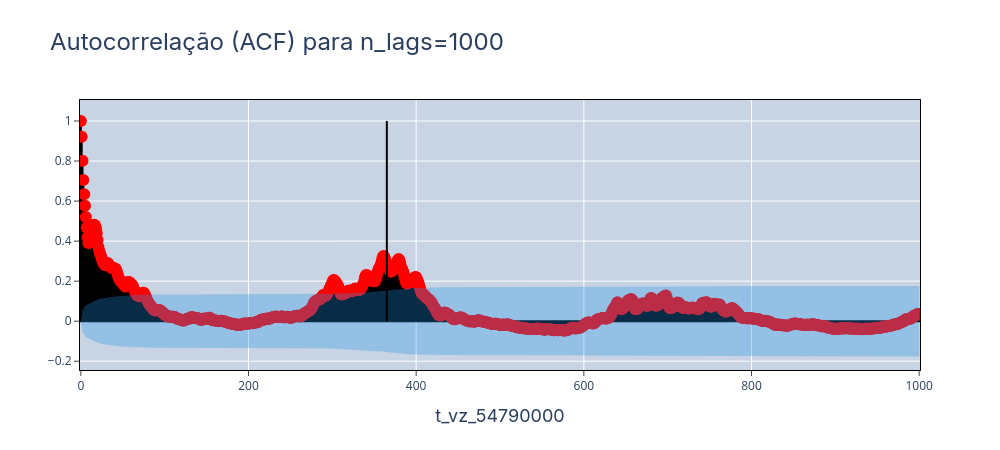
\includegraphics[scale=0.33]{Figuras/acf_jequitinhonha.png}
	\caption{Autocorrelação para a vazão do rio Jequitinhonha (fonte: o autor)}
	\label{fig:acf_jequitinhonha}
\end{figure}

\begin{figure}[!h]
	\centering
	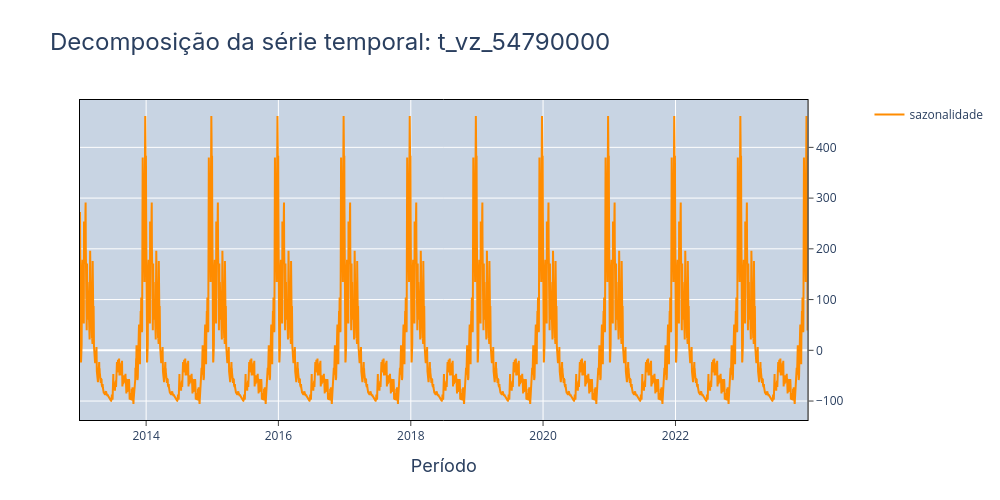
\includegraphics[scale=0.33]{Figuras/sazonalidade_jequitinhonha.png}
	\caption{Componente sazonal da série de vazão do rio Jequitinhonha (fonte: o autor)}
	\label{fig:sazonalidade_jequitinhonha}
\end{figure}

\begin{figure}[!h]
	\centering
	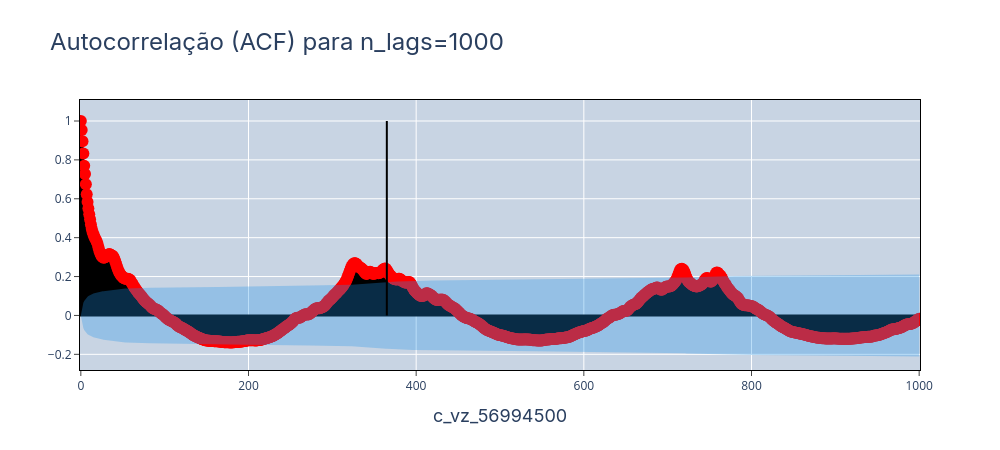
\includegraphics[scale=0.33]{Figuras/acf_rio_doce.png}
	\caption{Autocorrelação para a vazão do rio Doce (fonte: o autor)}
	\label{fig:acf_rio_doce}
\end{figure}

\begin{figure}[!h]
	\centering
	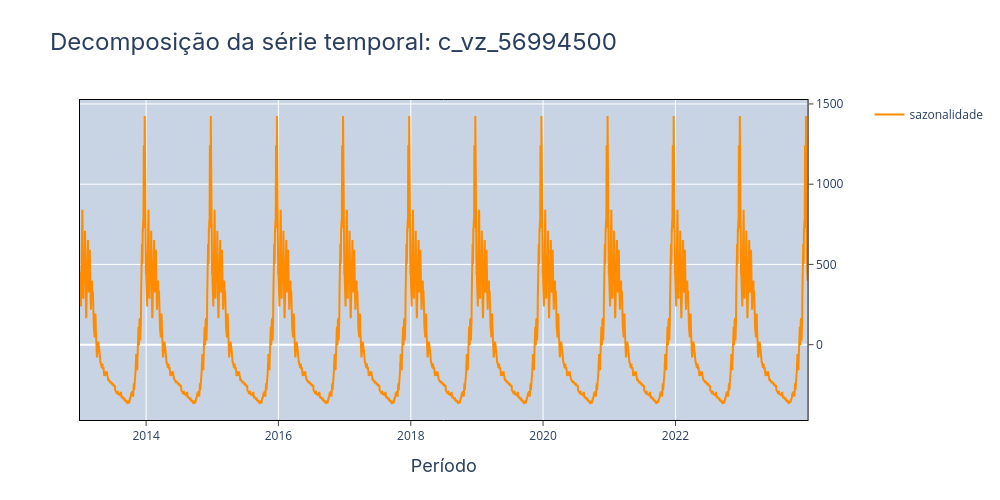
\includegraphics[scale=0.33]{Figuras/sazonalidade_rio_doce.png}
	\caption{Componente sazonal da série de vazão do rio Doce (fonte: o autor)}
	\label{fig:sazonalidade_rio_doce}
\end{figure}

\begin{figure}[!h]
	\centering
	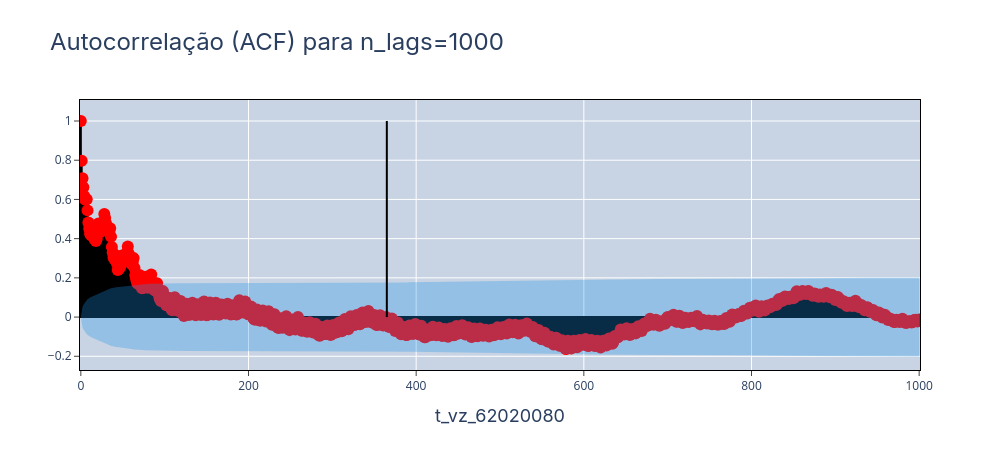
\includegraphics[scale=0.33]{Figuras/acf_rio_grande.png}
	\caption{Autocorrelação para a vazão do rio Grande (fonte: o autor)}
	\label{fig:acf_rio_grande}
\end{figure}

\begin{figure}[!h]
	\centering
	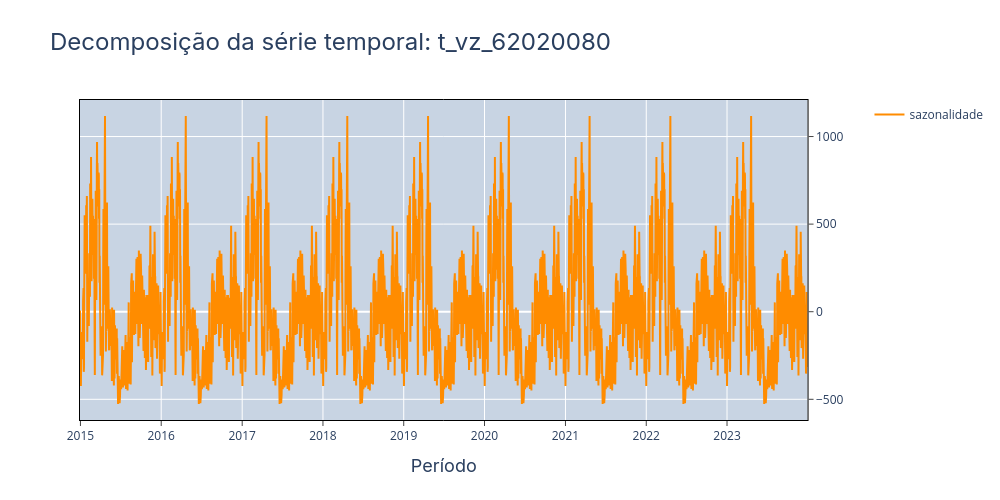
\includegraphics[scale=0.33]{Figuras/sazonalidade_rio_grande.png}
	\caption{Componente sazonal da série de vazão do rio Grande (fonte: o autor)}
	\label{fig:sazonalidade_rio_grande}
\end{figure}

\begin{figure}[!h]
	\centering
	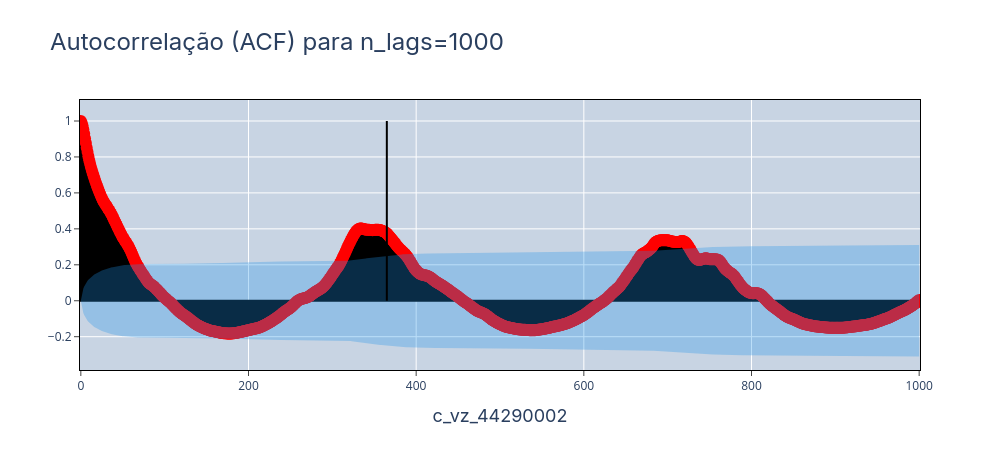
\includegraphics[scale=0.33]{Figuras/acf_rio_sao_francisco.png}
	\caption{Autocorrelação para a vazão do rio São Francisco (fonte: o autor)}
	\label{fig:acf_rio_sao_francisco}
\end{figure}

\begin{figure}[!h]
	\centering
	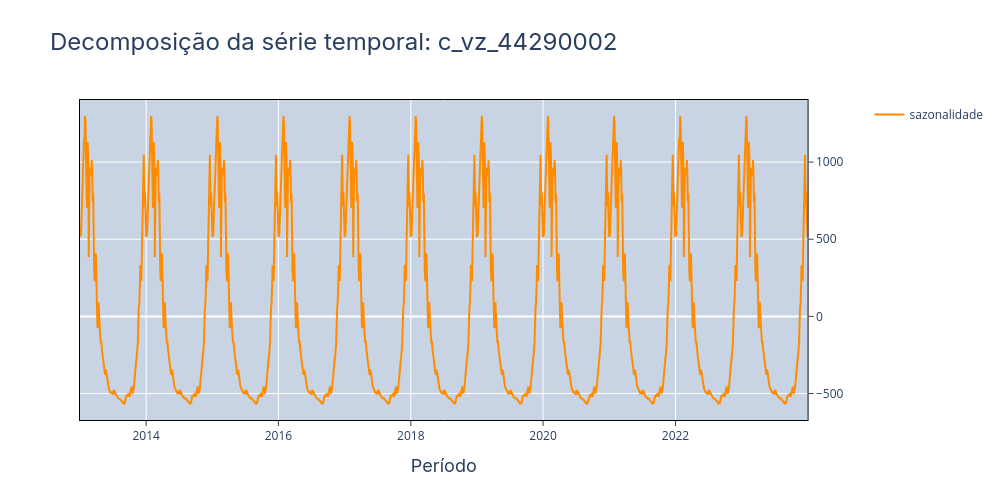
\includegraphics[scale=0.33]{Figuras/sazonalidade_rio_sao_francisco.png}
	\caption{Componente sazonal da série de vazão do rio São Francisco (fonte: o autor)}
	\label{fig:sazonalidade_rio_sao_francisco}
\end{figure}

As séries, digamos, mais bem comportadas, foram as séries do rio Doce e São Francisco. A decomposição sazonal para o rio Jequitinhonha apresentou ruído, mas a sazonalidade está caracterizada.

A análise incluiu também verificar estacionariedade das séries. Apesar de não terem sido aplicados modelos estatísticos no trabalho, por exemplo o ARIMA, a estacionariedade, quando presente, dá indícios importantes para qualquer modelo que venha ser utilizado. Quando uma série é caracterizada como estacionária implica dizer que suas propriedades estatísticas como a média, variância e autocorrelação ficam constantes ao longo do tempo. Isso melhora a convergência dos modelos e a previsibilidade.

Para este estudo foi aplicado um teste ADF (\textit{Augmented Dickey-Fuller} - Dickey-Fuller Aumentado) em que um valor-p (\textit{p-value}) menor ou igual a 0,05 (<= 0,05) confirmaria a estacionariedade. A biblioteca sktime tem um método pra isso e foi utilizado.\cite{loning2019sktime}
\todo[inline]{preciso explicar isso melhor, mas falta inspiração}

Outra característica a se investigar foi quanto à presença de ``cauda longa'' nos dados de precipitação e vazão. Este comportamento costuma estar presente em dados ambientais desta natureza.\cite{elena_macdonald_2023}

``Cauda longa'' refere-se a uma distribuição de frequência em que uma grande parte da população de eventos ocorre em uma região longe do ``centro'' ou da média da distribuição. Em uma distribuição normal, uma quantidade expressiva dos eventos concentra-se em torno da média, com menos ocorrências nas extremidades (as caudas). No entanto, na cauda longa, essas extremidades podem conter uma quantidade significativa de eventos, que somados podem representar uma fração relevante do total. Existe todo um campo de análise estatística especificamente dedicado ao estudo de cauda longa, que consegue lidar com baixa frequência mas de elevada magnitude, contudo estes não foram discorridos neste trabalho. Aqui interessaria apenas verificar a presença do fenômeno e como tratar.

A mitigação do efeito de cauda longa favorece modelos como a Regressão Linear, pois este assume uma distribuição normal dos dados, e neste sentido, a distribuição assimétrica dos eventos poderia comprometer a convergência. Os modelos de \textit{boosting} utilizados neste trabalho não seriam impactados pelo efeito de cauda longa, eles conseguem captar relações não-lineares e complexas satisfatoriamente, mas como se busca uma apresentação padronizada dos dados para os modelos, o tratamento aplicado para usar com a Regressão Linear será também empregado para os outros modelos.

Como de antemão já é sabido que possuem dados zerados, aplicar a transformação do logaritmo natural (ln(.)) não seria possível porque este cálculo não é definido para valores zero. Eis que foi aplicada a transformação ``log1p(.)'' da biblioteca NumPy \cite{numpyref}, que adiciona 1 ao valor a ser transformado para evitar o erro de logaritmo de zero.

Este procedimento conformou a cauda longa nos dados de vazão, como pode ser visto nas figuras REF_JEQUITI_1, REF_JEQUITI_2, REF_RIODOCE_1, REF_RIODOCE_2, REF_RIOGRANDE_1, REF_RIOGRANDE_2, REF_SAOFRANCISCO_1 e REF_SAOFRANCISCO_2.



\section{Modelos de Aprendizado de Máquina}
%Apresentar os modelos de ML utilizados (SeasonalNaive, LinearRegression, CatBoost e LightGBM) e justificativas.

\subsection{Seasonal Naive}

O modelo \textbf{Seasonal Naive} não pode ser considerado um modelo de previsão sofisticado. Em vez disso, ele funciona como uma linha de base (baseline), servindo como ponto de partida para avaliar o desempenho de outros modelos de previsão. Este modelo simplesmente repete a sazonalidade observada no período anterior, ou seja, assume que o comportamento do próximo ciclo sazonal será o mesmo do anterior, com um possível ajuste por \textit{drift} (desvio).

Esse método é útil para fornecer uma idéia inicial do comportamento esperado, permitindo que os modelos subsequentes sejam comparados a ele. Por ser um modelo simples, ele não captura tendências ou variações complexas, mas estabelece um \textit{benchmark} mínimo para o qual outros métodos mais elaborados e complexos devem se comparar.

\subsection{Regressão Linear}

O modelo de Regressão Linear (\textit{Linear Regression}) é uma abordagem estatística simples, porém poderosa, que busca modelar o relacionamento entre uma variável dependente e uma ou mais variáveis independentes através de uma linha reta. 

O funcionamento da Regressão Linear envolve o cálculo de coeficientes para as variáveis independentes, que determinam o peso de cada uma destas variáveis na previsão da variável dependente. O objetivo do modelo é minimizar o erro quadrático médio, ou seja, a soma dos quadrados das diferenças entre os valores previstos e os valores reais.

Os resultados obtidos com este modelo mostraram-se muito bons, e na verdade, ele se destacou como um modelo-base robusto para os outros modelos mais complexos. Sua simplicidade e eficácia tornam-no uma escolha bastante sólida. Isso será discutido.

Aqui está o fluxograma para o funcionamento do modelo de Regressão Linear

\todo[inline]{INSERIR DIAGRAMA ?}

\subsection{CatBoost e LightGBM}

Estes dois modelos são descritos juntos pois o funcionamento de ambos se baseia no mesmo princípio: ambos algoritmos constroem modelos fracos de árvores de decisão (\textit{decision tree}) de forma sequencial, onde cada árvore sucessiva é treinada para corrigir os erros da árvore anterior. Contudo, o LightGBM adota uma estratégia denominada ``Leaf-wise Growth'' ao invés da forma de construção tradicional ``Level-wise Growth''. Nesta estratégia, o crescimento ocorre folha a folha, a árvore expande as folhas com a maior redução de erro, resultando em árvores mais profundas e precisas. O revés nessa estretégia é que fica mais suscetível a \textit{overfitting}, mas existem parâmetros no modelo algoritmo que cuidam para que isso seja evitado. O CatBoost, por sua vez, adota uma estratégia denominada ``Ordered Boosting'', em que a construção das árvores se dá de maneira sequencial, porém não se usa todos os dados disponíveis para esta construção. Os dados de treinamento são ordenados de maneira aleatória e apenas partições destes dados são utilizados no processo. Por trabalhar sempre com uma amostra dos dados de treinamento, e a apresentação aleatória destes dados ao modelos, o CatBoost tem resiliência ao \textit{overfitting}, mas parâmetros que realizam ajustes nas árvores de decisão também podem ser empregados.

%\begin{figure}[!h]
%	\centering
%	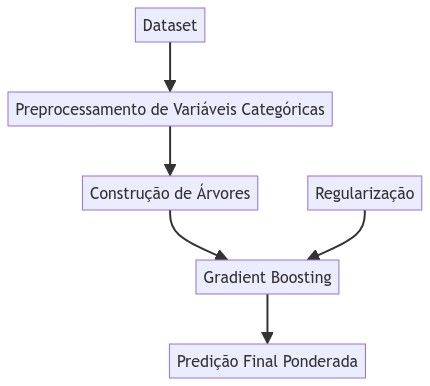
\includegraphics[scale=0.75]{Figuras/boosting_diagrama.jpg}
%	\caption{Diagrama resumindo o funcionamento dos modelos de \textit{boosting} (fonte: o autor)}
%	\label{fig:boosting_diagrama}
%\end{figure}

A escolha do algoritmo certo para um problema de previsão desta natureza depende das características dos dados e dos objetivos do estudo. O SeasonalNaive, embora simples, é um importante ponto de referência inicial. O modelo de Regressão Linear serve como uma \textit{baseline} confiável devido à sua eficácia e simplicidade. Já os modelos CatBoost e LightGBM foram opções mais avançadas, capazes de lidar com a complexidade dos dados e oferecer previsões precisas e eficientes. A comparação entre todos estes modelos permitiu que se escolhesse a abordagem que melhor atendesse às necessidades específicas da previsão de vazões.

%\section{Métricas de Avaliação}
%Listar as métricas usadas para avaliar o desempenho dos modelos (MAPE, RMSE, PBias* e KGE não-paramétrico**).
%(*: PBias ajuda a ver se o modelo está subestimando as previsões ou superestimando)
%(**: KGEnp (não paramétrico) é uma métrica comum e muito consagrada na hidrologia. Ela tem resiliência a outliers ao avaliar a qualidade do modelo)

%\section{Treinamento e Validação dos Modelos}
%Detalhar os procedimentos de treinamento e validação dos modelos.

\section{Modelo Proposto}
% Detalhar os procedimentos de treinamento e validação dos modelos.
\begin{figure}[!h]
	\centering
	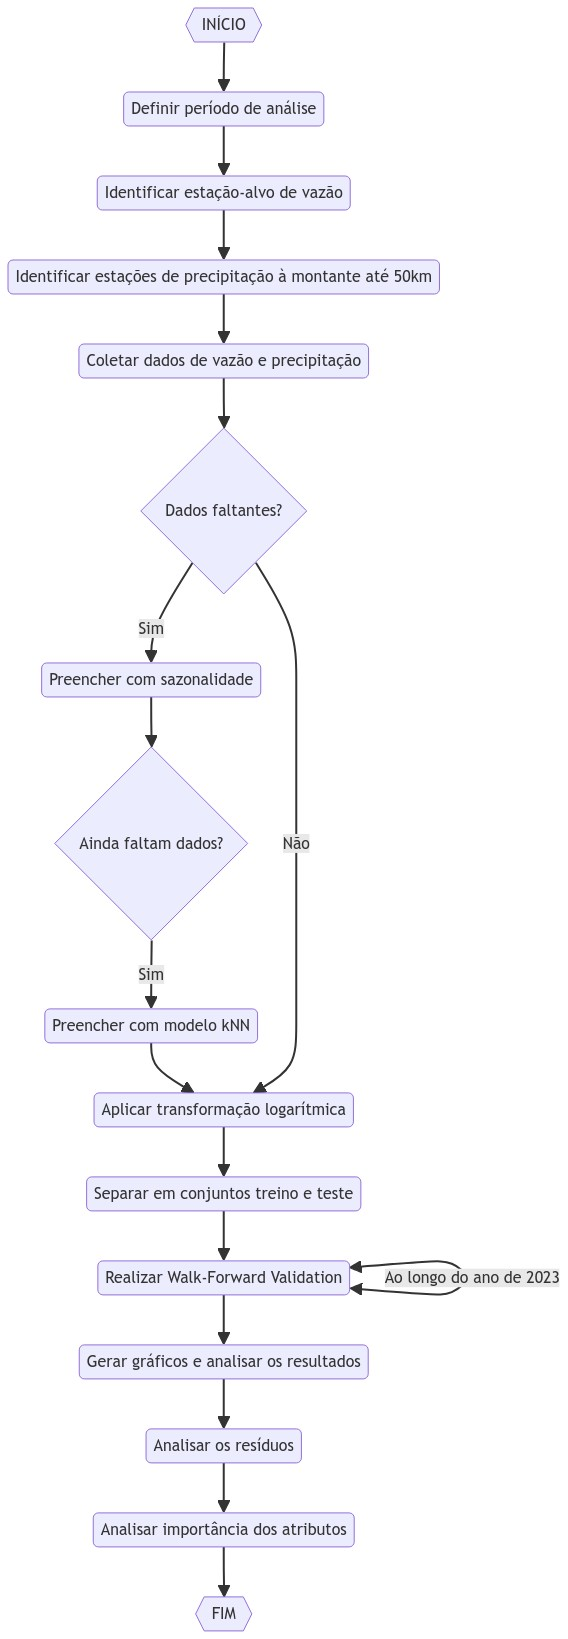
\includegraphics[scale=0.4]{Figuras/flowchart.png}
	\caption{Fluxo de trabalho (fonte: o autor)}
	\label{fig:fluxo_trabalho}
\end{figure}

